\documentclass[chaparabic,ceng,ms,12pt,oneandhalf,fivejury]{metu}
\usepackage{appendix}
\usepackage{longtable}
\usepackage[pdftex]{hyperref}
\usepackage[all]{hypcap}
\usepackage{todonotes}
\usepackage{graphicx}
\graphicspath{ {./images/} }
\usepackage[figuresright]{rotating}
\usepackage{xy} 
\usepackage{booktabs}
\usepackage{pifont}
\usepackage{color}
\usepackage{listings}
\usepackage{pdfpages}
\usepackage{array}
\usepackage{algorithm}
\usepackage{algorithmic}
\usepackage{float}
\usepackage{caption}
\usepackage{lastpage}
\usepackage{afterpage}
\usepackage{lipsum}
\usepackage{adjustbox}
\usepackage{rotating}

% \usepackage{graphicx}
\usepackage{amsmath,amssymb} % define this before the line numbering.
% \usepackage{ruler}
\usepackage{color}
% \usepackage{cite}
% \usepackage[utf8x]{inputenc}
% \usepackage{footnote}
% \makesavenoteenv{tabular}
% \makesavenoteenv{table}

\renewcommand{\sectionautorefname}{\S}
\renewcommand{\subsectionautorefname}{\S}

\newcommand{\norm}[1]{\left\lVert#1\right\rVert}

\captionsetup{belowskip=12pt,aboveskip=8pt}
\newcommand{\tab}{\hspace*{2em}}
\DeclareGraphicsExtensions{.pdf,.png,.jpg}


\usepackage{amsmath}
\usepackage{siunitx}
\usepackage{textcomp}
\usepackage{subcaption}


\usepackage{tikz}
\usepackage{mathtools}
% \usepackage{rotating}
%\PassOptionsToPackage{figuresright}{rotating}

\DeclarePairedDelimiter\ceil{\lceil}{\rceil}
\DeclarePairedDelimiter\floor{\lfloor}{\rfloor}


\newcommand{\EA}[1]{\textcolor{red}{[EA: #1]}}

% Name and Surname
\author{Ahmet Kürşad Şaşmaz}
% Thesis Title English and Turkish
\title{METU Thesis Template}
\turkishtitle{ODTÜ Tez Şablonu}

\date{January 2027}
 
% prof : Prof. Dr.
% assocprof : Assoc. Prof. Dr.
% assistprof : Assist. Prof. Dr.
% dr : Dr.
%
% Director of Institute
\director[prof]{Name Surname}
% Head of Department
\headofdept[prof]{Name Surname}
%
% Supervisor : English and Turkish
\supervisor[prof]{Ahmet Oğuz Akyüz}
% \turkishsupervisor{  } %if you will hard-code the academic title
%
% Affiliation of Supervisor in English and possibly in Turkish
\departmentofsupervisor{Computer Engineering, METU}

%\cosupervisor[dr]{Itır Önal Ertuğrul}
%\departmentofcosupervisor{Robotics Institute, Carnegie Mellon University}
%
% Committee Members
% In general members are sorted according to their academic titles
%
% Proffesors (1)
% Associate Professors (2)
% Assistant Professors (3)
% Other (4)
% 
% IMPORTANT:  All affiliatons should fit in a single line
% If affiliation line is broken into two lines you should shorten the affiliation by using 
% abbrevations or any other means
%
% First committee member should be the chair of examining committee
% Typically the chair is one of the highest ranked committee members
% Ask your supervisor if you are not sure
\committeememberi[assistprof]{Name Surname}
\affiliationi{Computer Engineering, METU}
% Second committee member is always your supervisor
\committeememberii[assistprof]{Name Surname}
\affiliationii{Computer Engineering, METU}

% IMPORTANT: If you are Ph.D. student your co-supervisor can not be in your 
% examination committee.

% \def\@proftitlename{Prof. Dr.}\def\@tproftitlename{Prof. Dr.}
% \def\@assocproftitlename{Assoc. Prof. Dr.}\def\@tassocproftitlename{Doç. Dr.}
% \def\@assistproftitlename{Assist. Prof. Dr.}\def\@tassistproftitlename{Yrd. Doç. Dr.}
% \def\@drtitlename{Dr.}\def\@tdrtitlename{Dr.}

\committeememberiii[assistprof]{Name Surname}
\affiliationiii{Computer Engineering, Bilkent University}
% Fourth committee member
\committeememberiv[assistprof]{Gülşah Tümüklü Özyer}
\affiliationiv{Computer Engineering, Atatürk University}
% Fifth committee member
\committeememberv[assistprof]{Jüri}
\affiliationv{JüriBölüm, Ankara University}

% The date of your thesis defence should be in DD.MM.YYYY format
\thesisdefencedate{01.01.2000}

%
% Keywords : English & Turkish, Comma seperated
\keywords{Keyword 1, Keyword 2, Keyword 3, Keyword 4, Keyword 5.  (Max 5 keywords)}
\anahtarklm{Anahtar Kelime 1, Anahtar Kelime 2, Anahtar Kelime 3, Anahtar Kelime 4, Anahtar Kelime 5. (En fazla 5 anahtar kelime)}
%
% Abstract in English
%
\abstract{
 Abstract in English [Max 250 words]
}
%
% Turkish Abstract
%
\oz{
 Tez Özeti [En fazla 250 kelime]
} 
%
% Dedication 
\dedication{Countless people have touched my heart and shaped what I have become today. \\ To the ones who kept their faith in me.}
%
%
% Acknowledgements   
\acknowledgments{
Acknowledgments [ Max 300 words] 
}

%
% End of Personal and Introductory Information
%%%%%%%%%%%%%%%%%%%%%%%%%%%%%%%%%5
\hypersetup{colorlinks=true, linkcolor=black, citecolor=black, urlcolor=blue}
\begin{document}
% Preliminaries
\begin{preliminaries}
% If you are willing to use any custom stuff before Chapters, put it here
% Such as List of Abbreviations
% Check the abbreviations.tex for a template list of abbreviations

\begin{theglossary}{LONGESTABBRV}

\item [ABRREVIATONS]
\item[] 

\item[2D] 2 Dimensional
\item[3D] 3 Dimensional 

\end{theglossary}

% End of Preliminaries
\end{preliminaries}
%   
% Latex content Goes Here 
% 
%

\setlength{\parindent}{0em}
\setlength{\parskip}{10pt}

% You can add as many chapters
% CHAPTER 1
\chapter{Introduction}
\label{chp:introduction}

\section{Motivation and Problem Definition}


\section{Proposed Methods and Models}


\section{Contributions and Novelties}


\section{The Outline of the Thesis}

% CHAPTER 2
\chapter{Background Knowledge}
\label{chp:background_knowledge}

\section{Perception}
\label{sec:perception}

\subsection{Human Visual System}
\label{subsec:human_visual_system}

The human visual system can be examined in three major sections : the eye, the retina and the neural structure in the brain. In this study, the main focus is the cells in the retina. These cells, named as cones, are the crucial part of the construction and the perception of the colors.

Stimulation of the cone cells has different sensitivity for each wavelength. The sensitivities of the cone cells with respect to wavelength are plotted in Figure~\ref{fig:lms_cone_normalized_sensitivities} These are the three types of cone cells, which are called with an abbreviation of their classifications according to their peak sensitive wavelengths:
\begin{itemize}
    \item $\mathbf{L}$ (Long, $\lambda_{max}$ = 565nm)
    \item $\mathbf{M}$ (Medium, $\lambda_{max}$ = 545nm)
    \item $\mathbf{S}$ (Short, $\lambda_{max}$ = 440nm)
\end{itemize}

\begin{figure}
    \centering
    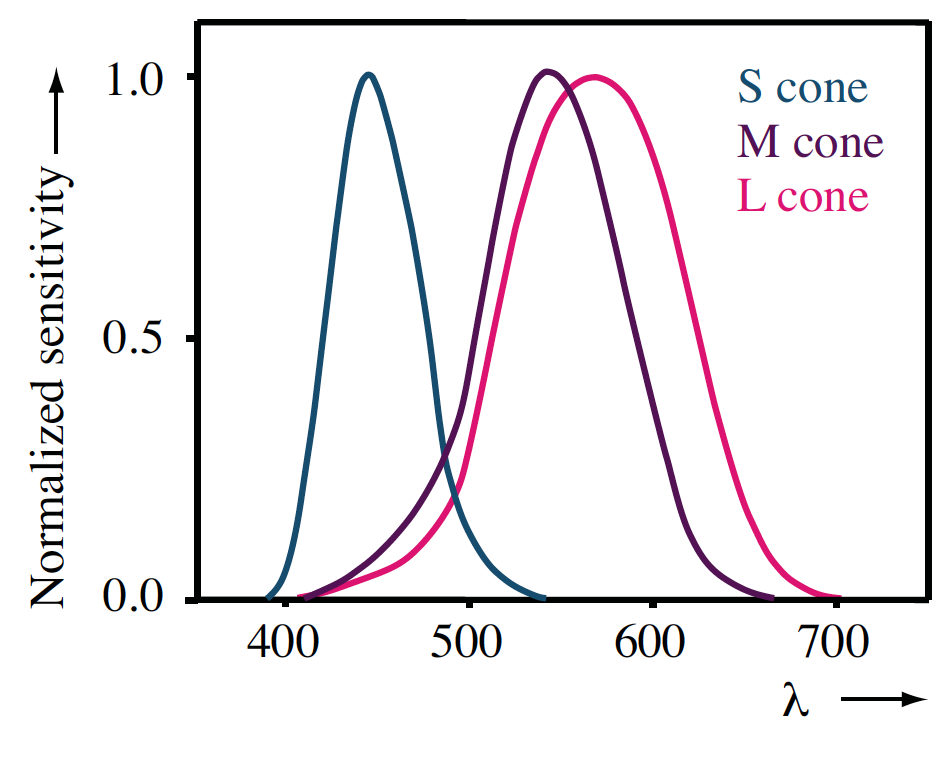
\includegraphics[width=0.5\linewidth]{figures/lms_cone_normalized_sensitivities.png}
    \caption{The normalized sensitivities of the three cone types \textit{Source:}~\cite{reinhard2008color}}
    \label{fig:lms_cone_normalized_sensitivities}
\end{figure}

\subsection{Reflectance and Illumination}
\label{subsec:reflectance_and_illumination}

A light can interact with an object in three ways: absorption, transmission and reflection. Every material has its own absorption, transmission and reflection function with respect to wavelength that sum to unity due to the conservation of energy. Absorbed, transmitted and reflected spectrum of light is just the multiplication of the spectrum of light with the material's absorption, transmission and reflection functions respectively.

Only the transmitted and reflected light can be perceived by human sensory system as the light incidents to the retina cells. Transmitted light is generally omitted or considered as reflected light in the study of chromatic adaptation. As a result, we will express the incident light $\mathbf{E}(\lambda)$ in the Eq.~\ref{eq:incident_light_formula} as the multiplication of the light function $\mathbf{I}(\lambda)$ and the material's reflection function $\mathbf{R}(\lambda)$ where $\lambda$ is the wavelength and it belongs to the visible spectrum $\mathbf{\Lambda}$. The visual representation of this equation is showed in Figure`\ref{fig:reflection_and_illumination}.

\begin{equation}
\mathbf{E}(\lambda) = \mathbf{I}(\lambda) \mathbf{R}(\lambda), \lambda \in \mathbf{\Lambda}
\label{eq:incident_light_formula}
\end{equation}

\begin{figure}
    \centering
    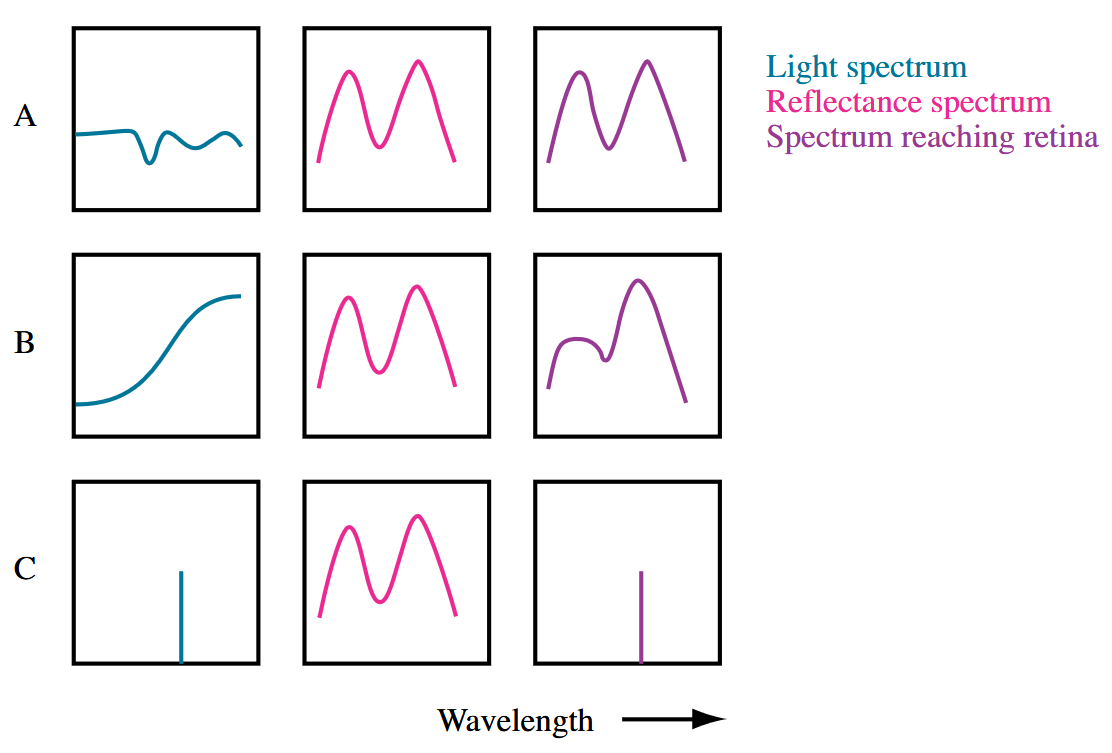
\includegraphics[width=0.8\linewidth]{figures/reflection_and_illumination.png}
    \caption{Visual representation of the multiplication of the light and the material's reflectance function in the Eq.~\ref{eq:incident_light_formula} \textit{Source:}~\cite{reinhard2008color}}
    \label{fig:reflection_and_illumination}
\end{figure}

\subsubsection{Dichromatic Reflection Model}
\label{sec:dichromatic_reflection_model}
Dichromatic reflection model analyzes the path of the reflected light in detail. The model separates the reflected light into two components: specular reflection and diffuse reflection.

The light that is immediately reflected after interacting with the material is not absorbed by the material. This type of light carries the information about the light source and it is named as specular reflection. The light that enters the object, exits from the surface without being absorbed by the object and scatters in every direction carries the information about the material and it is named as diffuse reflection. Therefore, the incident light to the retina carries the information of both and the incident light to retina model explained in Eq.~\ref{eq:incident_light_formula} is updated as Eq.~\ref{eq:dichromatic_incident_light_formula} where $\mathbf{R}_s(\lambda)$ and $\mathbf{R}_d(\lambda)$ represents the specular reflection and diffuse reflection respectively.

\begin{equation}
\mathbf{E}(\lambda) = \mathbf{I}(\lambda) (\mathbf{R}_s(\lambda) + \mathbf{R}_d(\lambda)), \lambda \in \mathbf{\Lambda}
\label{eq:dichromatic_incident_light_formula}
\end{equation}

Decomposing the terms $\mathbf{R}_s(\lambda)$ and $\mathbf{R}_d(\lambda)$ becomes important from the perspective of the study of illumination estimation.

\subsection{Camera Model}
\label{subsec:camera_model}

Modern digital cameras have three major components: the lens, the sensor and the image signal processor. The focus of this study covers the sensor and white balance correction step in the pipeline of image signal processing.  White balance correction step is explained in more detail in the following section \ref{sec:chromatic_adaptation_and_white_balance} of this chapter. The sensor is the crucial part where the light is captured for each of its primitive color components as energy and converted into electric current. The formula of the camera sensor model is given in Eq.~\ref{eq:camera_model_formula}. The incident light is filtered by proper color of the color filter array and then the light interacts with the sensor material, which generates electric current depending on its quantum efficiency with respect to the wavelength of the light.

The term $I_c$, an integration of the multiplication of some spectral distribution functions on the visible spectrum, represents the pixel value of the channel $c$ where $c \in \{R,G,B\}$ and $R,G,B$ are the abbreviations of the primary colors of the color filter array: red, green and blue. $\mathbf{E}(\lambda)$ represents the total energy of the incident light with respect to wavelength during the exposure which is explained in the Eq.~\ref{eq:incident_light_formula} in the section~\ref{subsec:reflectance_and_illumination}. $\mathbf{C}_c(\lambda)$ represents the transmitting proportion of the related filter of the color filter array with respect to wavelength. $\mathbf{Q}(\lambda)$ represents the quantum efficiency of the sensor material with respect to wavelength. Generally, the multiplication of $\mathbf{C}_c(\lambda)$ and $\mathbf{Q}(\lambda)$ is unique for every camera sensor and considered as a single component of the equation that is showed as $\mathbf{S}_c(\lambda)$ where $S$ represents the sensor sensitivity for the channel $c$. Finally, expanding the equation of $\mathbf{E}(\lambda)$, we acquire the core equation (Eq.~\ref{eq:camera_model_formula_sensor_sensitivity}) that will be used through this study.

\begin{subequations}
\label{eq:camera_model_formula}
\begin{align}
I_c = \int_{\mathbf{\Lambda}} \mathbf{E}(\lambda) \mathbf{C}_c(\lambda) \mathbf{Q}(\lambda) \, d\lambda \label{eq:camera_model_formula_separated} \\
I_c = \int_{\mathbf{\Lambda}} \mathbf{E}(\lambda) \mathbf{S}_c(\lambda) \, d\lambda \label{eq:camera_model_formula_sensor_sensitivity} \\
I_c = \int_{\mathbf{\Lambda}} \mathbf{I}(\lambda) \mathbf{R}(\lambda) \mathbf{S}_c(\lambda) \, d\lambda \label{eq:camera_model_formula_pixel}
\end{align}

\end{subequations}

\section{Chromatic Adaptation \& White Balance}
\label{sec:chromatic_adaptation_and_white_balance}

The color of the illuminant hitting the surface changes the observed color of the surface in a non-decomposable manner as can be derived from the section~\ref{subsec:reflectance_and_illumination}. However, human visual system can identify the object and its color under different lighting conditions by naturally removing the effect of the light source. This is known as color constancy~\cite{reinhard2008color}. In a specific manner, a white surface appears white to the human visual system under different light conditions as well. White balance is defined as the process of replicating this adaptation of human perception. 

\section{von Kries Coefficient Law}
\label{sec:von_kries_coefficient_law}

Johannes von Kries, in 1878, introduced a linear chromatic adaptation formula, as known as von Kries Coefficient Law, that is still used as an effective way of correcting the white balance. As explained in detail by MacAdam~\cite{MacAdamChromaticAdaptationVonKriesExplained1981}, von Kries defines the adaptation process as a multiplication of cone responses with a gain factor. In addition, this process becomes more coherent with the idea of independent channel adaptation. As a result, we obtain a linear diagonal transformation in the Eq.~\ref{eq:von_kries_lms}.

\begin{equation}
    \begin{bmatrix} 
    L_c \\ 
    M_c \\ 
    S_c 
    \end{bmatrix} = 
    \begin{bmatrix} 
    \alpha & 0 & 0 \\ 
    0 & \beta & 0 \\ 
    0 & 0 & \gamma 
    \end{bmatrix} 
    \begin{bmatrix} 
    L \\ 
    M \\ 
    S 
    \end{bmatrix}
    \label{eq:von_kries_lms}
\end{equation}

$L_c,M_c,S_c$ are the adapted cone responses with the coefficients $\alpha, \beta, \gamma$. The law states that the observer can see the object as the object is under an other light source if the per channel sensor response ratio is multiplied with the sensor response of the reflected light from the object. The statement is explained as an equation in Eq.~\ref{eq:von_kries_statement}.

\begin{equation}
    \begin{bmatrix} 
    L_2 \\ 
    M_2 \\ 
    S_2 
    \end{bmatrix} = 
    \begin{bmatrix} 
    \frac{L_2}{L_1} & 0 & 0 \\ 
    0 & \frac{M_2}{M_1} & 0 \\ 
    0 & 0 & \frac{S_2}{S_1} 
    \end{bmatrix} 
    \begin{bmatrix} 
    L_1 \\ 
    M_1 \\ 
    S_1 
    \end{bmatrix}
\label{eq:von_kries_statement}
\end{equation}

The terms $L_1, M_1, S_1$ represents the per channel sensor responses from the reflected light from the object with an arbitrary light. The terms $L_2, M_2, S_2$ represents the per channel sensor responses from the reflected light from the object with an other arbitrary light.

This equation explains that how the cells in retina adapt to the new light source and preserve the observed chromaticity of the object under different light sources by applying gain coefficients per channel.

\subsection{Wrong von Kries}

The camera model explained in the section~\ref{subsec:camera_model} has its own sensor response functions per channel which are being aimed to be identical with the cone cells but are not able to be exactly identical due to industrial reasons. In addition, white balance correction procedure is applied on the linear raw image data which the color space is the sensor's color space in the image signal processing pipeline. These enforce us to apply von Kries Coefficient Law on a different color space rather than LMS color space where the method is truly valid. This application is named as "wrong von Kries" as explained in~\cite{reinhard2008color} and formulated as in the Eq.~\ref{eq:wrong_von_kries_rgb}.

\begin{equation}
    \begin{bmatrix} 
    R_c \\ 
    G_c \\ 
    B_c 
    \end{bmatrix} = 
    \begin{bmatrix} 
    \alpha & 0 & 0 \\ 
    0 & \beta & 0 \\ 
    0 & 0 & \gamma 
    \end{bmatrix} 
    \begin{bmatrix} 
    R \\ 
    G \\ 
    B 
    \end{bmatrix}
    \label{eq:wrong_von_kries_rgb}
\end{equation}

The terms $R_c,G_c,B_c$ and $R,G,B$ represent the corrected RGB color channel values and the original RGB color channel values respectively. The illumination estimation works explained in the following chapters~\ref{chp:related_works} and~\ref{chp:proposed_method} aim to find the coefficients $\alpha$, $\beta$ and $\gamma$ in the sensor's color space for white balance correction.
% CHAPTER 3
\chapter{Datasets and Metrics}
\label{chp:datasets_and_metrics}

\section{Datasets}

\subsection{SFU Gray Ball}

Ciurea and Funt~\cite{sfuGrayBall} published a dataset that they recorded a two hour video with a camrecorder whose model is Sony VX-2000 in 2003. The group mounted a matte gray ball to the right bottom of the camera perspective. The gray ball enables us to extract the information about the illumination in the environment. The dataset consists 11,346 frames with 360x240 resolution from the two hour video that is taken both indoor and outdoor. However, the frames are highly correlated due to being a frame from a sequence of the video. In addition, the images of the dataset are stored as non-linear and gamma corrected. A linearized version of reduced subset of 1,135 independent frames are used for evaluation.

\subsection{Cube++}

Ershov et al.~\cite{ershov2020cube} published a dataset with 4,890 raw 18-megapixel images that extends its predecessors Cube and Cube+. All images are captured with two cameras, Canon EOS 550D and 600D, which have the same sensor. The scenes of the dataset includes variety of both indoor and outdoor environments. SpyderCube is used for the extracting the information about the illumination of the environment.

\subsection{Shi's Re-processing of Gehler's Raw Dataset }

The Shi-Gehler dataset, is also named as ColorChecker Dataset, originally introduced by Gehler et al. \cite{gehler2008bayesian} and later reprocessed into linear form by Shi and Funt \cite{shi2010reprocessed}, is the most used dataset for the evaluation of illumination estimation studies. It contains 56 images from the camera Canon 1D and 482 images from the camera Canon 5D sum to 568 indoor and outdoor images. The scenes contain Macbeth ColorChecker for extracting the information of the light source in the scene. In 2018, Hemrit et al. ~\cite{Hemrit2018ColorCheckerError} figured out that the extraction of ground truth illumination has mistakes and proposed a rehabilitated version of the dataset.

\subsection{NUS8}

The NUS 8-camera dataset \cite{cheng2014illuminant} was designed to examine the cross-camera behavior of illuminant estimation algorithms. It consists 1,736 linear raw images that are taken in roughly 260 scenes, meaning that the dataset has approximately 210 images per camera. The dataset uses Macbeth ColorChecker to extract information about the light sources of the scene.

\subsection{LSMI}

The Large Scale Multi-Illuminant (LSMI) dataset \cite{kim2021lsmi} contains 7,486 images of more than 2,700 scenes illuminated by two or three light sources and captured by three different cameras ((Samsung Galaxy Note 20 Ultra, Sony $\alpha$9, and Nikon D810). The dataset provides pixel-wise ground-truth illumination maps together with the chromaticity of each individual illuminant and the per-pixel mixing ratio between them. The ground truth is obtained by capturing the same scene under different illumination combinations and computing the difference between the resulting images. Therefore, LSMI serves as a key resource for developing and evaluating spatially varying white-balance algorithms.

\subsection{INTEL-TAU}

Laakom et al.~\cite{intelTAU} published the INTEL-TAU dataset, which was the largest publicly available high-resolution dataset for illumination estimation at the time of its release. It consists of 7,022 images collected with three different camera sensors, Canon 5DSR, Nikon D810 and the mobile phone sensor Sony IMX135, and is organized into three subsets of 1,466 indoor, 2,327 outdoor and 3,229 close-up scenes. A SpyderCube color target, which exposes two gray surfaces facing different directions together with two white surfaces, is placed in each scene; the gray surfaces yield two separate ground truth illuminant records per image corresponding to the two directions, while the white surfaces are used to detect over-saturation. The dataset also applies privacy masking to sensitive content such as faces, making it compliant with the General Data Protection Regulation (GDPR).

\subsection{MIMO}

Beigpour et al.~\cite{mimoAndConditionalRandomFields} published the Multi-Illuminant Multi-Object (MIMO) dataset, which consists of 78 images captured under two non-uniformly distributed illuminants, split between a Laboratory set of controlled scenes and a Real-World set of everyday indoor and outdoor scenes containing simple and complex diffuse and specular objects. Unlike the datasets discussed above, every image, of size $302 \times 452$, is accompanied by a pixel-wise ground truth illumination image that stores the illuminant RGB vector for every pixel of the scene rather than a single global illuminant or a small number of per-region illuminants, which makes the dataset suitable for evaluating spatially varying illumination estimation methods directly at the pixel level.

\subsection{Rendered WB Dataset}

Afifi et al.~\cite{afifiRenderedWB} published the Rendered WB dataset together with a method for correcting improperly white-balanced camera-rendered sRGB images, since such images have already been non-linearly processed by the camera pipeline and no longer preserve the raw sensor values needed by the classical illuminant estimation methods. The dataset consists of more than 65,000 pairs of images, each pair containing a scene rendered with an incorrect camera white balance setting alongside the same scene correctly white-balanced, spanning multiple camera models so that the generalization of a correction method to a camera unseen during training can be evaluated directly. Because the pairs are defined at the level of the final sRGB output rather than the raw illuminant chromaticity, the dataset targets the correction of white balance errors introduced anywhere in the camera rendering pipeline, rather than only the estimation of the scene illuminant itself.

\subsection{sRGB-LSMI}

Serrano-Lozano et al.~\cite{revisitingImageFusionRenderedWB} built the sRGB-LSMI dataset for the multi-illuminant image fusion task by repurposing the raw images of the LSMI dataset~\cite{kim2021lsmi}. Each raw scene is rendered into an sRGB image under five different white balance presets, resulting in more than 16,000 images that are used to train and evaluate fusion based white balance correction methods, which combine the differently rendered versions of the same image into the final corrected result. Unlike LSMI, whose ground truth is the raw pixel-wise illuminant chromaticity of the scene, the ground truth of sRGB-LSMI is the multi-illuminant white-balanced sRGB image itself, obtained in two steps: first, the white-balanced version of the single-illuminant image is computed using the color checker references of LSMI, then the per-pixel brightness of this corrected image is adjusted with an auto white balance corrected version of the original multi-illuminant image.

\subsection{Multi Illumination In The Wild}

Murmann et al.~\cite{multiIlluminationInTheWild} published a large-scale dataset of real, in-the-wild indoor scenes, each captured under 25 different lighting directions rather than a single fixed illuminant, containing more than 1,000 scenes for a total of over 25,000 high dynamic range images. Unlike the datasets discussed above, which provide one or a small number of ground truth illuminants for an otherwise static scene, this dataset varies the direction and the appearance of the light source itself across the captures of the same scene, which makes it suitable not only for illumination estimation but also for image relighting and mixed-illuminant white balance research.

\section{Metrics}

\subsection{Recovery Angular Error}

In the study of illumination estimation, the chromaticity of the light source is the important thing rather than the brightness of the light source. Because the incorrect thing about the captured image is chromatic tint. As a result, the metric compares the estimated chromaticity of the light source with the true chromaticity of the light source without considering the brightness. The evaluation is applied as the angle between the RGB vector of estimated light source and the RGB vector of true light source with the formula Eq.~\ref{eq:recovery_angular_error}.

\begin{equation}
    \epsilon_{recovery} = \arccos\left(\frac{L_{est} \cdot L_{gt}}{\norm{L_{est}} \norm{L_{gt}}}\right) \frac{180}{\pi}
    \label{eq:recovery_angular_error}
\end{equation}

The term $L_{est}$ and $L_{gt}$ represent the RGB vector of the estimated light source and the RGB vector of the true light source respectively.

\subsection{Reproduction Angular Error}

Finlayson et al.~\cite{finlaysonReproductionAngularError} proposed a new perspective to the evaluation with angular error in 2014. Accepting that a white surface reflects the light as it is, a white surface must have the same chromaticity with the true light source. As a result, the surface must be achromatic after applying von Kries as explained in the section~\ref{sec:von_kries_coefficient_law}.

For a specific angular error value, there are infinite number of RGB vectors for the estimated light source with respect to the RGB vector of true light source. However, all of these vectors will give different chromaticities for a corrected white surface.

The authors state that evaluating by using the angle between the RGB vector of corrected white surface and the desired achromatic RGB vector. The formula forms as in Eq.~\ref{eq:reproduction_angular_error}.

\begin{equation}
    \epsilon_{reproduction} = \arccos\left(\frac{\frac{L_{gt}}{L_{est}} \cdot \begin{bmatrix} 1 & 1 & 1 \end{bmatrix}^T} {\norm{\frac{L_{gt}}{L_{est}}} \norm{\begin{bmatrix} 1 & 1 & 1 \end{bmatrix}^T}}\right) \frac{180}{\pi}
    \label{eq:reproduction_angular_error}
\end{equation}

The term $L_{est}$ and $L_{gt}$ represent the RGB vector of the estimated light source and the RGB vector of the true light source respectively and the division is element-wise. Here, the $L_{gt}$ is the chromaticity of a white surface that reflects the true light source as it is.

\subsection{Mean Angular Error}

Extending the illumination estimation study from global illumination to spatially varying illumination requires evaluating the errors as pixel-wise. Therefore, we extend the recovery angular error and the reproduction angular error by taking the average of errors per pixels of the estimated illumination map and the true illumination map. The evaluation formulas for mean recovery angular error and mean reproduction error is in Eq.~\ref{eq:mean_recovery_angular_error} and Eq.~\ref{eq:mean_reproduction_angular_error} respectively.

\begin{equation}
    \epsilon_{\mu,recovery} = \frac{1}{\norm{\mathcal{P}}}\sum_{p\in\mathcal{P}}{\arccos\left(\frac{I_{p,est} \cdot I_{p,gt}}{\norm{I_{p,est}} \norm{I_{p,gt}}}\right) \frac{180}{\pi}}
    \label{eq:mean_recovery_angular_error}
\end{equation}

\begin{equation}
    \epsilon_{\mu,reproduction} = \frac{1}{\norm{\mathcal{P}}}\sum_{p\in\mathcal{P}}{\arccos\left(\frac{\frac{I_{p,gt}}{I_{p,est}} \cdot \begin{bmatrix} 1 & 1 & 1 \end{bmatrix}^T} {\norm{\frac{I_{p,gt}}{I_{p,est}}} \norm{\begin{bmatrix} 1 & 1 & 1 \end{bmatrix}^T}}\right) \frac{180}{\pi}}
    \label{eq:mean_reproduction_angular_error}
\end{equation}

The term $I_{p,est}$ and $I_{p,gt}$ represent the RGB vector of the pixel $p$ of the estimated illumination map and the RGB vector of the pixel $p$ of the true illumination map respectively.

\subsection{$\mathbf{\Delta}$E2000}
Both of the angular error metrics measure the deviation between two RGB vectors in the device dependent sensor space, which is not perceptually uniform. Consequently, two estimations having exactly the same angular error may produce color distortions of very different magnitude for a human observer, depending on the region of the color space they fall into. Since the ultimate purpose of the illumination estimation is to obtain an image that looks correct to a human, an evaluation that is aligned with the human perception is also required. For this purpose, we use the CIEDE2000 color difference formula~\cite{luoDevelopmentCIEDE2000}, which is defined in the CIELAB color space and which weights the lightness, the chroma and the hue differences separately in order to compensate the perceptual non-uniformity of the CIELAB space.

Let $(L^*_1, a^*_1, b^*_1)$ and $(L^*_2, a^*_2, b^*_2)$ denote the CIELAB coordinates of the two colors that are compared. The formula first modifies the $a^*$ axis so that the neutral colors are handled consistently, as given in Eq.~\ref{eq:ciede2000_primes}.
\begin{equation}
    \begin{gathered}
        C^*_i = \sqrt{a^{*2}_i + b^{*2}_i}, \quad \bar{C}^* = \frac{C^*_1 + C^*_2}{2}, \quad
        G = \frac{1}{2}\left(1 - \sqrt{\frac{\bar{C}^{*7}}{\bar{C}^{*7} + 25^7}}\right) \\
        a'_i = (1 + G)\,a^*_i, \quad C'_i = \sqrt{a'^2_i + b^{*2}_i}, \quad h'_i = \arctan_2\left(b^*_i, a'_i\right)
    \end{gathered}
    \label{eq:ciede2000_primes}
\end{equation}
The lightness, chroma and hue differences are then computed as in Eq.~\ref{eq:ciede2000_differences}, where the hue difference is expressed as a chord length so that it is comparable with the other two terms.
\begin{equation}
    \Delta L' = L^*_2 - L^*_1, \quad
    \Delta C' = C'_2 - C'_1, \quad
    \Delta H' = 2\sqrt{C'_1 C'_2}\sin\left(\frac{\Delta h'}{2}\right)
    \label{eq:ciede2000_differences}
\end{equation}
The weighting functions $S_L$, $S_C$ and $S_H$ scale these differences according to the position of the color pair in the space, and the rotation term $R_T$ accounts for the interaction between the chroma and the hue differences in the blue region, as formulated in Eq.~\ref{eq:ciede2000_weights}.
\begin{equation}
    \begin{gathered}
        S_L = 1 + \frac{0.015\left(\bar{L}' - 50\right)^2}{\sqrt{20 + \left(\bar{L}' - 50\right)^2}}, \quad
        S_C = 1 + 0.045\,\bar{C}', \quad
        S_H = 1 + 0.015\,\bar{C}'T \\
        T = 1 - 0.17\cos\left(\bar{h}' - 30^\circ\right) + 0.24\cos\left(2\bar{h}'\right) + 0.32\cos\left(3\bar{h}' + 6^\circ\right) - 0.20\cos\left(4\bar{h}' - 63^\circ\right) \\
        R_T = -2\sqrt{\frac{\bar{C}'^7}{\bar{C}'^7 + 25^7}}\,\sin\left(60^\circ\exp\left(-\left(\frac{\bar{h}' - 275^\circ}{25}\right)^2\right)\right)
    \end{gathered}
    \label{eq:ciede2000_weights}
\end{equation}
The terms $\bar{L}'$, $\bar{C}'$ and $\bar{h}'$ are the arithmetic means of the corresponding values of the two colors, the mean hue being taken with respect to the $360^\circ$ wrap-around. Finally, the color difference is obtained as in Eq.~\ref{eq:ciede2000}, where the parametric factors are set to $k_L = k_C = k_H = 1$ for the reference viewing conditions.
\begin{equation}
    \Delta E_{00} = \sqrt{\left(\frac{\Delta L'}{k_L S_L}\right)^2 + \left(\frac{\Delta C'}{k_C S_C}\right)^2 + \left(\frac{\Delta H'}{k_H S_H}\right)^2 + R_T\frac{\Delta C'}{k_C S_C}\frac{\Delta H'}{k_H S_H}}
    \label{eq:ciede2000}
\end{equation}

Following the same reasoning with the reproduction angular error, we apply the metric on a white surface that is corrected by the estimated light source. The corrected white surface is mapped to the CIELAB space and it is compared with the reference white, which is the desired appearance of that surface. The evaluation is given in Eq.~\ref{eq:delta_e2000_error}.
\begin{equation}
    \epsilon_{\Delta E} = \Delta E_{00}\left(\Phi\left(\frac{L_{gt}}{L_{est}}\right), \Phi\left(\begin{bmatrix} 1 & 1 & 1 \end{bmatrix}^T\right)\right)
    \label{eq:delta_e2000_error}
\end{equation}
The term $\Phi(\cdot)$ denotes the transformation from the linear RGB values to the CIELAB coordinates, which is performed through the CIE XYZ space with the D65 reference white, and the division is element-wise. Since the brightness of the light source is not a part of the estimation problem, the corrected white surface is normalized to have the same luminance with the reference white before the transformation. In this way the lightness difference $\Delta L'$ vanishes and only the chromatic deviation contributes to the reported error.

As in the case of the angular errors, the metric is extended to the spatially varying illumination by averaging the color difference over the pixels of the illumination map, as formulated in Eq.~\ref{eq:mean_delta_e2000_error}.
\begin{equation}
    \epsilon_{\mu,\Delta E} = \frac{1}{\norm{\mathcal{P}}}\sum_{p\in\mathcal{P}}{\Delta E_{00}\left(\Phi\left(\frac{I_{p,gt}}{I_{p,est}}\right), \Phi\left(\begin{bmatrix} 1 & 1 & 1 \end{bmatrix}^T\right)\right)}
    \label{eq:mean_delta_e2000_error}
\end{equation}
The term $I_{p,est}$ and $I_{p,gt}$ represent the RGB vector of the pixel $p$ of the estimated illumination map and the RGB vector of the pixel $p$ of the true illumination map respectively.
% CHAPTER 4
\chapter{Related Works}
\label{chp:related_works}

\section{Introduction}
\label{sec:related_works_introduction}

 The study of illumination estimation can be separated into two major levels of illumination estimation. Firstly, relying on the fact that most of the photographs taken by people have a simple environment where the light sources can be regarded as a single light source due to negligible variance. The process of estimating the illumination and applying white balance algorithms on these images gives well enough results when only the major light source of the scene is considered. In this study, this type of illumination estimation algorithms are named as "Global Illumination Estimation" or "Single Illumination Estimation" and discussed at the section~\ref{sec:global_illumination_estimation}. Secondly, more analysis about the light sources and their interactions with the scene is required when the scene is complex in terms of illumination. For example, a complex scene has a multiple light sources where they have different chromaticities and have variable effect on the different regions of the scene. In this study, this type of illumination estimation algorithms are named as "Spatially Varying Illumination Estimation" or "Mixed Illumination Estimation" and discussed at the section~\ref{sec:spatially_varying_illumination_estimation}.

\section{Global Illumination Estimation}
\label{sec:global_illumination_estimation}

Global illumination estimation, or single illumination estimation, focuses on finding the chromaticities of the most effective light source in the scene. Then, white balance correction algorithms apply the same illuminant for all pixels of the image. The datasets have a single ground truth illuminant and the evaluation benchmark is built on comparing the estimated illuminant chromaticities with the ground truth illuminant chromaticities.

The related works about global illumination estimation can be collected in three main approaches: statistical approaches, gamut based approaches and learning based approaches.

\subsection{Statistical Approaches}
\label{sec:statistical_approaches}

Statistical approaches in global illumination estimation studies are focuses on finding the effective illuminant by making an assumption about the scene and extracting information about the illuminant after analyzing the image with statistical approaches.

\subsubsection{Gray World}
\label{algorithm:gray_world}
The Gray World hypothesis, as proposed by Buchsbaum (1980) assumes that the average surface reflectance in a scene is chromatic under a neutral illuminant~\cite{gray_world}. Under this assumption, any deviation in the observed average channel values is due to the influence of the light source. The illuminant chromaticity is estimated by calculating the mean intensity of each color channel, and the adaptation coefficients are derived as follows:

\[
\left( \frac{\bar{I}_G}{\bar{I}_R}, \,\, 1, \,\, \frac{\bar{I}_G}{\bar{I}_B} \right)
\]

While the Gray World algorithm is computationally efficient and have a good performance in scenes with high variety of chromaticity, it results color cast when the surface reflectances of the scene is not distributed equally. For example, vast region of wall with flat color dominates other chromaticities and causes color cast. Furthermore, the scenes with less hue diversity results with achromatic corrected images. For example, a picture of forest, full of green, causes a grayscale output when the image is corrected with the illuminant estimated by this algorithm.

\subsubsection{White Patch (Max-RGB)}
\label{algorithm:white_patch}
The White Patch hypothesis, also known as the Max-RGB algorithm in practice, was proposed by Brainard and Wandell (1986)~\cite{white_patch} within the context of the Retinex Theory proposed by Land (1977) ~\cite{retinex}. This hypothesis assumes that the maximum intensity in each color channel is a clue of a perfectly reflective surface, in other words, a white patch that totally reflects the light source. Under this assumption, the chromaticity of the illuminant is estimated by the maximum values of each channel and the adaptation coefficients are derived as follows:

\[
\left( \frac{G_{max}}{R_{max}}, \,\, 1, \,\, \frac{G_{max}}{B_{max}} \right)
\]

While the proposed method is computationally trivial and gives better results for the scenes that has less chromatic diversity when comparing with Gray World ~\ref{algorithm:gray_world}, the accuracy of the algorithm is highly depends on the presence of an achromatic reflector in the scene. Also, the performance of the algorithm is affected by highly reflective mono-chromatic materials, causes to biased peak values for a specific channel. Furthermore, the method is highly sensitive to sensor noise and over-saturated pixels.

\subsubsection{Shades of Gray}
\label{algoritm:shades_of_gray}
The Shades of Gray hypothesis, was proposed by Finlayson and Trezzi (2004) \cite{shades_of_gray}, generalizes the Gray World and White Patch assumptions into a single framework by representing them with Minkowski norm. The $p$-th order average provides a framework that covers assumptions from Gray World (with $p=1$) to White Patch ($p \to \infty$). Under this assumption, the chromaticity of the illuminant is estimated by the $p$-th order average of each color channel, defined as:

\begin{equation}
\|c\|_p = \left( \frac{1}{N} \sum_{i=1}^{N} c_i^p \right)^{1/p}
\end{equation}

where $N$ is the total number of pixels. The adaptation coefficients are then derived as:

\[
\left( \frac{\|G\|_p}{\|R\|_p}, \,\, 1, \,\, \frac{\|G\|_p}{\|B\|_p} \right)
\]

The primary challenge in applying the Shades of Gray algorithm lies in the empirical selection of the optimal $p$-norm, because the ideal value varies significantly depending on the scene content and sensor characteristics. The literature frequently cites $p=6$ for natural images but this value is not optimal for every case. A lower $p$ value increases the influence of all pixels, causes to the same color casts in the Gray World algorithm ~\ref{algorithm:gray_world}. Conversely, as $p$ increases, the norm becomes more sensitive to high-intensity values, eventually inheriting the vulnerability of the Max-RGB approach ~\ref{algorithm:white_patch} to sensor noise and clipping. Consequently, the performance of the algorithm is sensitive to this hyperparameter, often requiring calibration or scene-adaptive selection.

\subsubsection{Gray Edge}
\label{algorithm:gray_edge}

The Gray Edge hypothesis, as proposed by van de Weijer et al. (2007), extends the Minkowski norm framework ~\ref{algoritm:shades_of_gray} by assuming that the average of the image gradients is achromatic \cite{gray_edge}. To reduce the sensitivity of derivatives to local noise, the image is first convolved with a Gaussian filter of scale $\sigma$. The illuminant is then estimated using the $p$-th order Minkowski norm of the $n$-th order derivatives of each color channel:

\begin{equation}
\| \nabla^n I_{\sigma,c} \|_p = \left( \sum_{i=1}^{N} \left| \frac{\partial^n I_{\sigma,c}}{\partial x^n} (i) \right|^p \right)^{1/p}
\end{equation}

where $I_{\sigma,c} = I_c * G_{\sigma}$ represents the convolution of the image channel with a Gaussian kernel. The compensation is then applied by taking the coefficients as follows:

\[
\left( \frac{\| \nabla^n I_{\sigma,G} \|_p}{\| \nabla^n I_{\sigma,R} \|_p}, \,\, 1, \,\, \frac{\| \nabla^n I_{\sigma,G} \|_p}{\| \nabla^n I_{\sigma,B} \|_p} \right)
\]

Despite its ability to outperform pixel-based methods by focusing on reflectance changes at object boundaries, the Gray Edge algorithm ~\ref{algorithm:gray_edge} is highly sensitive to the selection of its hyperparameters ($n$, $p$, and $\sigma$). The method primarily fails in scenes with insufficient geometric structure or low contrast, where sharp edges are absent, causing the derivative values to be dominated by sensor noise rather than actual reflectance transitions. Additionally, the presence of "chromatic aberrations" or "demosaicing artifacts" can introduce artificial gradients that bias the illuminant estimation.

\subsubsection{Local Space Average Color}
\label{algorithm:local_space_average_color}
Ebner (2009) observes that the Gray World assumption ~\ref{algorithm:gray_world} is imposed on the entire image although the illuminant frequently varies across the scene, and proposes to apply the same assumption locally by computing a space average color for every pixel \cite{ebnerLocalSpaceAverageColor}. The averaging is carried out on a grid of processing elements, one per pixel, which iteratively exchange their estimates with their neighbors:
\begin{equation}
a'_c(x) = \frac{1}{\norm{\mathcal{N}(x)}} \sum_{x' \in \mathcal{N}(x)} a_c(x'), \qquad
a_c(x) = p \, I_c(x) + (1 - p) \, a'_c(x)
\end{equation}
where $\mathcal{N}(x)$ is the set of the elements neighboring the pixel $x$ and the parameter $p$ controls the extent of the averaging. The iteration converges to a weighted average of the surrounding pixels whose support grows as $p$ decreases, and the global space average color of the Gray World algorithm ~\ref{algorithm:gray_world} is obtained in the limit. Assuming that the reflectance of the local neighborhood averages to gray, the local illuminant is estimated as $2a_c(x)$, and the correction is applied per pixel according to the von Kries coefficient law explained in the section~\ref{sec:von_kries_coefficient_law}:
\begin{equation}
o_c(x) = \frac{I_c(x)}{2 a_c(x)}
\end{equation}
The author additionally considers a variant in which the component of the local space average color orthogonal to the gray vector is subtracted from the pixel, which shifts the color instead of scaling it. Since an estimate is produced for every pixel, the output is directly an illumination map, therefore the method addresses the spatially varying illumination without any additional stage. On the other hand, the gray world assumption is now imposed on every neighborhood, so a uniformly colored region that is larger than the support of the averaging is pushed towards gray and loses its saturation. The extent parameter $p$ has to be selected with respect to the resolution of the image, and it trades this desaturation against the loss of the locality. Furthermore, the averaging is isotropic and smooth, hence the estimate cannot follow a sharp illumination boundary such as a shadow edge and it diffuses the two illuminants into each other, and a small $p$ requires a large number of iterations to converge.

\subsubsection{Weighted Gray Edge}
\label{algorithm:weighted_gray_edge}
Gijsenij et al. (2012) argue that not every edge is equally informative for the illuminant, and extend the Gray Edge framework ~\ref{algorithm:gray_edge} by weighting the derivatives according to their photometric origin \cite{weightedGrayEdge}. Following the dichromatic reflection model explained in the section~\ref{sec:dichromatic_reflection_model}, a specular edge is generated by the term $\mathbf{R}_s(\lambda)$, which is independent of the material and therefore varies along the color of the light source, whereas a shadow-shading edge is generated by the term $\mathbf{R}_d(\lambda)$ and varies along the color of the surface itself, carrying no information about the illuminant. The edges are classified by projecting the spatial derivative onto the photometric directions defined by the current illuminant estimate $\hat{e}$:
\begin{equation}
\hat{c}_f = \frac{I_{\sigma}}{\| I_{\sigma} \|}, \qquad
\hat{c}_i = \frac{\hat{e}}{\| \hat{e} \|}, \qquad
\hat{c}_h = \frac{\hat{e} \times I_{\sigma}}{\| \hat{e} \times I_{\sigma} \|}
\end{equation}
which correspond to the shadow-shading, specular and hue variations respectively. A weight $w$ is assigned to each pixel with respect to the resulting edge type and inserted into the Minkowski norm of the derivatives:
\begin{equation}
\| w \nabla^n I_{\sigma,c} \|_p = \left( \sum_{i=1}^{N} \left| w(i) \frac{\partial^n I_{\sigma,c}}{\partial x^n} (i) \right|^p \right)^{1/p}
\end{equation}
and the compensation coefficients are taken as follows:
\[
\left( \frac{\| w \nabla^n I_{\sigma,G} \|_p}{\| w \nabla^n I_{\sigma,R} \|_p}, \,\, 1, \,\, \frac{\| w \nabla^n I_{\sigma,G} \|_p}{\| w \nabla^n I_{\sigma,B} \|_p} \right)
\]
Since the projection directions depend on the unknown illuminant, the estimation is repeated iteratively until the change in the estimate becomes negligible, and the choice $w = 1$ reduces the method to the Gray Edge algorithm ~\ref{algorithm:gray_edge}. The reported best performance is obtained by emphasizing the specular edges, which is consistent with $\mathbf{R}_s(\lambda)$ following the color of the illuminant. On the other hand, the method relies on the actual presence of informative edges, so it provides little benefit for matte scenes and it degrades when the highlights are clipped by the sensor. The iterative scheme also inherits the quality of its initialization, as a biased initial estimate rotates the photometric directions and reinforces its own error, and the hyperparameters $n$, $p$ and $\sigma$ remain in addition to the weighting parameters.

\subsubsection{Bright Pixels}
\label{algorithm:bright_pixels}

The Bright Pixels approach, introduced by Joze et al. (2012), is based on the observation that certain pixels in an image carry more significant information about the illuminant than others \cite{bright_pixels}. Unlike global statistical methods that process the entire image, this method posits that pixels with higher luminance values are more likely to reflect the true color of the light source accurately.

In practical implementations and comparative benchmarks, this approach is often simplified by selecting pixels whose luminance exceeds a predefined threshold. The estimated illuminant $I$ for each channel $c$ is typically calculated as the arithmetic mean of this brightest pixel set $\mathcal{P}_{bright}$:
\begin{equation}
I_c = \frac{\sum_{i \in \mathcal{P}_{bright}} I_c(i)}{|\mathcal{P}_{bright}|}
\end{equation}
However, the method faces significant challenges when the brightest elements in a scene are not achromatic but highly saturated, such as vivid colorful light sources or bright reflective surfaces. In such cases, the algorithm incorrectly attributes the surface color to the illuminant. Furthermore, like the White Patch hypothesis \ref{algorithm:white_patch}, this approach remains sensitive to sensor clipping and overexposure, where saturated pixels can lead to a heavily biased estimation. Additionally, by focusing exclusively on the most intense regions, the model may overlook secondary light sources in multi-illuminant scenarios.

\subsubsection{Bright and Dark Pixels via PCA}
\label{algorithm:bright_pixels_pca}

The Bright-and-Dark Pixel method, proposed by Cheng et al. (2014) \cite{cheng2014illuminant}, uses both the brightest and the darkest pixels to estimate the illuminant. The idea is that the light color is easier to find from colors that lie far apart in the color space. Rather than using image edges to obtain such colors, this method picks them directly from the color distribution. It ranks pixels not by their raw brightness, but by how close each color is to the mean color direction $I_0$ of the image (the Gray World average). For a pixel $I(x)$, this projection distance $d_x$ is:
\begin{equation}
d_x = \frac{I(x) \cdot I_0}{\|I(x)\|\,\|I_0\|}
\end{equation}
where $\|\cdot\|$ is the Euclidean norm. The pixels are sorted by $d_x$; the top $n\%$ are kept as bright pixels $\mathcal{P}_{bright}$ and the bottom $n\%$ as dark pixels $\mathcal{P}_{dark}$. The illuminant $\hat{e}$ is then the first PCA vector of these selected pixels only:
\begin{equation}
\hat{e} = \mathrm{PCA}_1\big(\mathcal{P}_{bright} \cup \mathcal{P}_{dark}\big)
\end{equation}

The lowest error is reported at $n = 3.5\%$ in the literature. Adding dark pixels to bright ones reduces the error for many images.

This method is fast and needs no training. However, it fails when a scene has only one or two colors: the colors then form a single line, so the PCA vector points to the surface color instead of the light. It also works poorly under unusual red or blue light, and the result depends on the chosen value of $n$.

\subsubsection{Grey Pixels}
\label{algorithm:grey_pixels}
Rather than imposing a statistical assumption on the whole image, Yang et al. (2015) propose to detect the pixels that are physically informative about the light source, namely the achromatic surfaces, which reflect the illuminant as it is \cite{yangGrayPixels}. The reflectance of a grey surface is spectrally flat, hence the response reduces to $I_c(x) = R(x) e_c$ where $R$ is common to the three channels, and taking the logarithm turns the illuminant into an additive constant per channel. Consequently, a local contrast operator eliminates the contribution of the light source and yields the same response in every channel:
\begin{equation}
\delta_c(x) = \left| \nabla \left( \log \left( I_c * G_{\sigma} \right) (x) \right) \right|, \quad c \in \{R, G, B\}
\end{equation}
The deviation among the channel contrasts is then used as a measure of greyness, and the pixels having the smallest values are collected into the set $\mathcal{G}$:
\begin{equation}
GI(x) = \sqrt{\frac{1}{3} \sum_{c} \left( \delta_c(x) - \bar{\delta}(x) \right)^2}, \qquad \bar{\delta}(x) = \frac{1}{3} \sum_{c} \delta_c(x)
\end{equation}
The illuminant is estimated by averaging the responses of the selected pixels, and the compensation coefficients are taken as follows:
\begin{equation}
\hat{e}_c = \frac{1}{\norm{\mathcal{G}}} \sum_{x \in \mathcal{G}} I_c(x), \qquad \left( \frac{\hat{e}_G}{\hat{e}_R}, \,\, 1, \,\, \frac{\hat{e}_G}{\hat{e}_B} \right)
\end{equation}
Since the greyness is defined per pixel, the selected pixels can also be grouped spatially, which allows the method to be applied to the scenes illuminated by more than one light source. On the other hand, the measure responds to any surface whose reflectance is locally constant, so a uniformly colored surface under shading produces an equally low index and biases the estimation towards the color of that surface. The method further requires grey surfaces to be present in the scene, and the near-flat and saturated regions have to be discarded beforehand, because their contrast is dominated by sensor noise and clipping rather than by the actual intensity variation. Finally, the performance depends on the scale $\sigma$ and on the proportion of the pixels that are selected as grey.

\subsubsection{Double-Opponency}
\label{algorithm:double_opponency}
Rather than starting from a statistical assumption about the scene, Gao et al. (2015) build the estimation upon the color processing stages of the human visual system, and observe that the color distribution of the responses of the double-opponent (DO) cells of the primary visual cortex to a color-biased image coincides with the direction of the light source \cite{gaoDoubleOpponency}. Following the opponent organization of the visual pathway, a yellow channel $I_Y = (I_R + I_G)/2$ and a luminance channel $I_{Lum} = I_R + I_G + I_B$ are constructed first, and the input is transformed into the single-opponent space:
\begin{equation}
O_{rg} = \frac{I_R - I_G}{\sqrt{2}}, \qquad
O_{by} = \frac{I_Y - 2 I_B}{\sqrt{6}}, \qquad
O_{l} = \frac{I_{Lum}}{\sqrt{3}}
\end{equation}
The receptive field of a single-opponent cell is modeled by a Gaussian, and a double-opponent cell is constructed from two single-opponent cells of opposite polarity having different scales, which corresponds to convolving each opponent channel with a difference of Gaussians:
\begin{equation}
DO_c(x) = O_c(x) \ast \left[ G_{\sigma}(x) - k \, G_{\lambda\sigma}(x) \right], \qquad c \in \{rg, by, l\}
\end{equation}
where $\sigma$ and $\lambda\sigma$ are the scales of the center and the surround, and the relative cone weight $k$ controls the contribution of the surround. A balanced cell with $k=1$ responds only to the color contrast, whereas an unbalanced one responds to the uniformly colored regions as well, so the parameter interpolates between an edge driven and a region driven behavior. The responses are then transformed back into the RGB space by the inverse of the opponent transformation, and the illuminant is obtained by pooling each channel separately with a sum or a max operator, followed by a normalization:
\begin{equation}
\hat{e}_c = \frac{\underset{x}{\text{pool}} \left( DO_c(x) \right)}{\sum_{c'} \underset{x}{\text{pool}} \left( DO_{c'}(x) \right)}, \qquad
\left( \frac{\hat{e}_G}{\hat{e}_R}, \,\, 1, \,\, \frac{\hat{e}_G}{\hat{e}_B} \right)
\end{equation}
Although the model is motivated physiologically, the two pooling alternatives inherit the corresponding weaknesses of the previous approaches, since the max operator is vulnerable to the clipping and the noise as in the White Patch algorithm ~\ref{algorithm:white_patch}, while the sum operator is biased by the large uniformly colored surfaces as in the Gray World algorithm ~\ref{algorithm:gray_world}. Moreover, the reported optimal cone weight differs considerably between the datasets, since a scene containing few edges requires the responses of the colored regions to be enhanced whereas a cluttered scene does not, and this makes the parameter selection dependent on the scene content together with the scale $\sigma$. Finally, the responses are pooled over the entire image, therefore a single illuminant vector is produced and the spatially varying illumination is not addressed.

\subsubsection{Fast White Balance Algorithm Based on Pixel Grayness}
\label{algorithm:fast_wb_grayness}

The Fast White Balance algorithm, as proposed by Thai (2017) \cite{fast_wb_greyness}, estimates the illuminant by calculating a weighted average of all pixels based on their "grayness" in the $YC_bC_r$ color space. This method is based on the premise that pixels closer to the achromatic (gray) point provide more reliable information about the illuminant than more saturated pixels. Each pixel $i$ is assigned a weight $w_i$ derived from its distance to the neutral point in the chroma plane ($C_b, C_r$), and the weighted average for each image channel $\bar{I}_c$ is calculated as:

\begin{equation}
w_i = \exp\left( -\frac{C_{b,i}^2 + C_{r,i}^2}{2\sigma^2} \right) \quad \bar{I}_c = \frac{\sum_{i=1}^{N} w_i I_c[i]}{\sum_{i=1}^{N} w_i}
\end{equation}

The compensation is applied by taking coefficients as following:

\[
\left( \frac{Y_{max}}{\bar{I}_R}, \frac{Y_{max}}{\bar{I}_G}, \frac{Y_{max}}{\bar{I}_B} \right)
\]

This approach effectively combines the statistical stability of the Gray World hypothesis \ref{algorithm:gray_world} with a non-linear weighting mechanism that prioritizes near-neutral surfaces. However, the performance of the algorithm is highly sensitive to the $\sigma$ parameter, which defines the "grayness" threshold; an overly restrictive $\sigma$ may exclude valuable data, while a loose $\sigma$ allows saturated colors to bias the estimation. A significant limitation arises in scenes with strong color casts, where the illuminant shifts the actual gray surfaces far from the $C_b=0, C_r=0$ origin, causing the algorithm to assign low weights to the most informative pixels. Furthermore, the use of $Y_{max}$ as a global scaling factor assumes that the peak luminance represents a neutral white, making the method vulnerable to monochromatic highlights and sensor clipping, which can lead to over-saturation or color shifts in the final output.

\subsubsection{Grayness Index}
\label{algorithm:grayness_index}
Qian et al. (2019) observe that the greyness measure of Yang et al. ~\ref{algorithm:grey_pixels} is derived from the Lambertian model, and therefore it frequently reports clearly colored pixels as grey, since the interaction between the terms $\mathbf{R}_s(\lambda)$ and $\mathbf{R}_d(\lambda)$ of the dichromatic reflection model explained in the section~\ref{sec:dichromatic_reflection_model} may also equalize the channel contrasts of a colored surface \cite{qianFindingGrayPixels}. Instead of comparing the channel contrasts with each other, the residual of each channel with respect to the luminance is taken in the log domain, and the local contrast operator $C\{\cdot\}$, realized by a Laplacian of Gaussian filter, is applied afterwards. Under the neutral interface reflection assumption both reflection terms of an achromatic surface are spectrally flat, hence this residual stays constant in a local neighborhood and its contrast vanishes. The deviation from this condition defines the index, where the green channel is redundant since the responses of the red and the blue channels rarely overlap:
\begin{equation}
GI(x) = \norm{\left[ C\{\log I_R - \log \norm{I}\}, \,\, C\{\log I_B - \log \norm{I}\} \right]}, \qquad \norm{I} = I_R + I_G + I_B
\end{equation}
The pixels having a local contrast below a threshold $\epsilon$ are discarded beforehand, so that a small index is produced by an achromatic surface under varying intensity rather than by a flat region carrying no spatial cue, and the resulting map is averaged in a local window to suppress the isolated responses caused by sensor noise. The illuminant is estimated by averaging the $N\%$ of the pixels with the smallest index, collected in the set $\mathcal{G}$, and the compensation coefficients are taken as follows:
\begin{equation}
\hat{e}_c = \frac{1}{\norm{\mathcal{G}}} \sum_{x \in \mathcal{G}} I_c(x), \qquad \left( \frac{\hat{e}_G}{\hat{e}_R}, \,\, 1, \,\, \frac{\hat{e}_G}{\hat{e}_B} \right)
\end{equation}
For the scenes containing more than one light source, the selected pixels are grouped into $M$ clusters by K-means and a separate estimate is computed per cluster, then the illumination map is obtained by combining these estimates with weights decaying with the distance of the pixel to the cluster centroids, which encourages the neighboring pixels to share a similar illuminant. On the other hand, the method still requires achromatic surfaces to be present in the scene, and it additionally requires them to exhibit an intensity variation, since the uniformly lit regions are removed by the contrast threshold. The neutral interface reflection and the narrowband sensor assumptions also have to hold, and the estimation depends on the proportion $N$ and the threshold $\epsilon$. Finally, the reported error distribution has a heavy tail, which indicates that the accuracy degrades considerably on the scenes where the detected pixels are few or where they are illuminated by different light sources.

\subsubsection{Degree-of-Linear-Polarization-Based Color Constancy}
\label{algorithm:dolp_color_constancy}

Ono et al. (2022) observe that the degree of linear polarization (DoLP) measured at an achromatic surface is largely independent of the chromaticity of the illuminant, and propose to use this physical cue, rather than a purely statistical or spectral assumption, to detect the achromatic pixels that are informative about the light source \cite{ono2022degree}. A polarization camera captures the DoLP alongside the RGB response of every pixel, and the pixels whose DoLP is consistent with a physically achromatic surface are selected independently of how saturated their observed color appears, even for surfaces that would be discarded as chromatic by the color based methods described above. The illuminant is then estimated by averaging the responses of the selected pixels, following the same reasoning as the grey pixel detection methods ~\ref{algorithm:grey_pixels}.

Since the method relies on a physical measurement rather than an assumption about the statistics of the scene, it remains accurate on the scenes where the color based achromatic pixel detectors are misled by a uniformly colored surface. However, the approach requires a polarization sensitive camera and is only valid under the assumptions of the underlying polarization model, namely that the observed light is either directly reflected or singly scattered, so the accuracy degrades for surfaces exhibiting complex subsurface scattering or multiple reflections. The method further depends on having a sufficient number of suitably oriented achromatic surfaces in the scene, in the same manner as the color based grey pixel detectors, and its benefit over these detectors is only realized when the additional polarization channel is available from the sensor.

\subsubsection{BIO-CC: Biologically Inspired Color Constancy}

Ulucan et al. (2022) build a hierarchical model that follows the structure of the human color perception pathway more closely than the earlier biologically motivated approaches, incorporating a non-uniform sampling of the image that mimics focal and peripheral vision, the retinotopic organization of the visual field, the response of double-opponent cells explained in the section~\ref{algorithm:double_opponency}, and a saliency map analogous to that of the visual cortex \cite{ulucan2022bio}. Each of these stages contributes a distinct processing step, and their outputs are pooled hierarchically to obtain the final illuminant estimate, rather than computing a single statistic over the whole image at once.

Since every stage of the pipeline is derived from a fixed characterization of the human visual system rather than fit to a training set, the model requires no training data, unlike the deep learning based methods described later in this section. The authors additionally show that the same hierarchical structure reproduces the perceptual color assimilation illusions observed in human vision, which the purely engineering driven statistical algorithms above are not designed to capture. On the other hand, since the model is a fixed pipeline of biologically motivated stages rather than a learned one, it cannot improve with additional training data, and the parameters that determine how the different stages are combined still have to be tuned by hand, which involves the same scene-dependent trade-offs as the single-stage statistical methods it builds upon.

\subsubsection{Block-Based Deviation of Salient Pixels}
\label{algorithm:block_based_salient_pixels}
Ulucan et al. (2023) combine the assumptions of the White Patch ~\ref{algorithm:white_patch} and the Gray World ~\ref{algorithm:gray_world} algorithms by assuming that every region of the scene contains at least one bright pixel and that the world is achromatic on average, so that the deviation of the brightest pixels from the achromatic value is caused by the light source \cite{ulucanSalientPixels}. Since the statistics of a scene are not uniform over the image, the estimation is not performed globally. After the darkest and the brightest pixels are clipped in order to suppress the noise, the image is divided into non-overlapping blocks $\mathcal{B}_p$, and each block is described by the maximum response of its channels together with its own achromatic reference:
\begin{equation}
I_{p,max} = \left[ \max_{x \in \mathcal{B}_p} I_R(x), \,\, \max_{x \in \mathcal{B}_p} I_G(x), \,\, \max_{x \in \mathcal{B}_p} I_B(x) \right], \qquad
\mu_p = \frac{1}{3 \norm{\mathcal{B}_p}} \sum_{x \in \mathcal{B}_p} \sum_{c} I_c(x)
\end{equation}
The deviation is expressed as a scaling vector $\mathbf{C}_p$ that maps the brightest response of the block onto its achromatic value, which is obtained by solving a non-negative least squares problem, and the illuminant is taken as the average of the estimates of the blocks:
\begin{equation}
\mathbf{C}_p = \underset{\mathbf{C}_p}{\arg\min} \norm{I_{p,max} \mathbf{C}_p - \mu_p}_2 \,\,\, \text{s.t.} \,\,\, c \geq 0 \,\,\, \forall c \in \mathbf{C}_p, \qquad
L_{est} = \frac{1}{n} \sum_{p=1}^{n} \mathbf{C}_p
\end{equation}
Not every element of a block carries information about the illuminant, and a block dominated by a region such as the sky biases its own estimate. Therefore only the salient pixels, which are defined as the pixels closest to white, are taken into account: a temporary estimate is produced from the channel means, the image is corrected with it, and the pixels whose angular error to the vector $\begin{bmatrix} 1 & 1 & 1 \end{bmatrix}^T$ remains below a threshold are retained. On the other hand, the size of the blocks has to be selected with respect to the resolution of the image, since a large size leaves too few blocks to capture the local statistics whereas a small size increases the chance of obtaining uniformly colored blocks, for which the gray world assumption does not hold. The performance also degrades when the statistical distribution is uniform throughout the image or when the scene contains no pixel close to white, which is a common weakness of the statistics based approaches. Finally, the estimates of the blocks are averaged into a single vector, hence the illumination is still assumed to be global despite the computation being local.

\subsubsection{Multi-Scale Salient Varying Local Spatial Statistics}
\label{algorithm:multi_scale_salient}
Ulucan et al. (2024) extend their block-based estimation ~\ref{algorithm:block_based_salient_pixels} by selecting the informative pixels explicitly and by repeating the computation over a scale space \cite{ulucanMultiScaleSalient}. The saliency is defined through the brightness, which is consistent with the observation that the human visual system may discount the illuminant by relying on the patches with the highest luminance: the image is transformed into the opponent space and the brightest pixels of the black-white channel $O_{BW}$ form a binary map $S$. Since the selected pixels do not contribute equally, a weight map is additionally derived from the same channel, and the informative image is obtained by modulating the input with both maps:
\begin{equation}
W(x) = 1 - \frac{1}{2\pi\sigma^2}\exp\left(-\frac{\left(O_{BW}(x) - \mu\right)^2}{2\sigma^2}\right), \qquad
I'(x) = I(x) \, W(x) \, S(x)
\end{equation}
where $\mu$ and $\sigma$ are the mean and the standard deviation of $O_{BW}$, and $W$ is normalized so that its elements sum to one. The informative image is then successively downsampled into $L$ levels, the number of which is adapted to the resolution of the image. At the finer levels the image is divided into non-overlapping blocks whose size is again determined by the resolution, whereas at the coarser levels the whole image is treated as a single region, since the blocks would otherwise contain too few distinct colors for the gray world assumption to hold. For every region the brightest response and the local achromatic value are extracted and the scaling vector $\mathbf{C}_P$ is obtained as in the section~\ref{algorithm:block_based_salient_pixels}, then the estimates are averaged within a scale and the scales are combined linearly:
\begin{equation}
\hat{L}_s = \frac{1}{n_s}\sum_{k=1}^{n_s} \mathbf{C}_{P_k}, \qquad
L_{est} = \frac{1}{L}\sum_{s=1}^{L} \hat{L}_s
\end{equation}
The authors further report that the accuracy of several existing algorithms improves when their computations are carried into the scale space in the same manner, and they outline an extension in which the estimates of the regions are kept separate rather than being averaged, which turns the method into a multi-illuminant approach. On the other hand, the assumptions of the White Patch ~\ref{algorithm:white_patch} and the Gray World ~\ref{algorithm:gray_world} algorithms are still imposed on every region, therefore the accuracy decreases as the color distribution of the scene becomes uniform throughout the image, and the selection is driven by the luminance alone, so a bright but strongly colored region such as the sky may still be marked as informative. The method also introduces further parameters, namely the proportion of the brightest pixels, the controlling parameter of the block size and the number of the levels, which are determined experimentally on the benchmarks. Finally, the scales are combined with equal weights and the estimates are collapsed into a single vector, hence a global illumination is assumed unless the outlined extension is applied.

\subsection{Gamut Based Approaches}
\label{sec:gamut_based_approaches}

Gamut based approaches in global illumination estimation studies are focuses on finding the effective illuminant by comparing the set of colors observed in the image with the set of colors that are known to be observable under a canonical light source. Since a light source restricts the colors that can be recorded by the camera, the mappings that place the observed set inside the canonical set form a feasible set of solutions, and the illuminant is estimated by selecting a single mapping from this set with a geometric criterion.

\subsubsection{The Theoretical Foundation of Gamut Mapping}
\label{algorithm:theoretical_foundation_of_gamut}

The color constancy method by Forsyth (1990) \cite{baseofgamut} changes the problem from simple statistics to geometry and linear algebra. Forsyth says that "the color of an object is its color under a fixed canonical light, rather than as a surface reflectance function." This idea is based on a physical rule: surfaces cannot reflect more light than they receive. The model uses the Mondriaan World as a base, assuming all surfaces are flat and Lambertian, with a single uniform light source and no shadows or extra reflections.

The algorithm, called Crule (Coefficient Rule), finds the light using these geometric steps:
\begin{enumerate}
\item \textbf{Canonical Gamut Construction:} Creating a shape (convex hull) of all possible colors under a standard white light.
\item \textbf{Observed Gamut:} Finding the shape of the colors actually present in the current image.
\item \textbf{Feasible Set Search:} Finding all diagonal matrix values that can fit the observed shape inside the canonical shape.
\item \textbf{Maximum Volume Heuristic:} Choosing the values that make the final colors in the image as bright and vivid as possible.
\end{enumerate}

This method is strong because it does not depend on the average color of the scene or the position of objects. However, its performance is limited by its strict assumptions. The flat-surface assumption means it struggles with real 3D objects that have shadows and complex lighting. Also, the method needs many different colors in the image to work well; if a scene has only one color, the geometric constraints are too weak to find the correct light. Finally, in very colorful lighting, camera noise can make the estimation difficult because the physical limits of the sensors are reached.

\subsubsection{Color Constancy in Diagonal Chromaticity Space}

The study by Finlayson (1996) \cite{diagonal_chromatography} improves Forsyth's gamut mapping by moving the problem from 3D RGB space to a 2D diagonal chromaticity space. Forsyth’s original CRULE algorithm \cite{baseofgamut} had strict physical requirements: surfaces had to be perfectly flat, and the light had to be uniform across the scene. Finlayson shows that these restrictions exist only because the old method tries to recover the full intensity (brightness) of colors. By using chromaticity (r/b,g/b), the algorithm removes intensity and focuses only on the orientation of color vectors, which allows it to work with real-world 3D objects and specular reflections.

The algorithm introduces a new geometric framework to solve the limitations of earlier models:
\begin{enumerate}
\item \textbf{Diagonal Chromaticity Mapping:} The 3D camera responses are mapped onto a 2D plane. Finlayson proves that in this space, color gamuts remain convex and light changes are still accurately described by a simple diagonal matrix.
\item \textbf{Sensor Sharpening:} To ensure the diagonal model is sufficient, the algorithm assumes or applies a sensor transformation. This is better than older non-diagonal 3×3 linear models—such as the one by Maloney and Wandell \cite{maloney_wandell_recover_surface_spectral} —which required complex statistical models for both light and surfaces.
\item \textbf{Illuminant Gamut Constraint:} A major addition is the "canonical illuminant gamut". Instead of considering every possible diagonal matrix, the algorithm only looks for mappings that correspond to real, physically possible light sources.
\end{enumerate}  

This method is more effective than the original CRULE because it combines surface constraints with illuminant constraints. By intersecting these two sets of possible solutions, the algorithm can find the correct light even in images with very few colors. However, the method still has some constraints; it works best when the camera sensors are "sharp" or can be mathematically sharpened to reduce errors to a minimum. While it handles 3D shapes and specularities better than Forsyth’s model, it still relies on the assumption that the light is spectrally constant across the scene.

\subsubsection{Improvements to Gamut Mapping}
\label{algorithm:improvements_to_gamut_mapping}

The study by Barnard (2000) \cite{barnardGamutMappingImproved} does not introduce a new gamut mapping framework, but instead improves the two separate stages that every gamut mapping algorithm consists of: constraining the set of possible solutions, and choosing a single solution from this feasible set. Barnard points out that the first stage completely depends on the diagonal model of illumination change, which is only an approximation and whose accuracy is a function of the camera sensors. When the diagonal model fails, the observed colors may not map into the canonical gamut with any diagonal transform at all, which produces an empty feasible set. Earlier solutions treated such empty intersections as measurement error and simply increased the error tolerances until a solution appeared, but this does not work for severe failures such as the ones caused by fluorescent surfaces.

The algorithm improves the classical framework with two modifications:
\begin{enumerate}
\item \textbf{Extended Canonical Gamut:} For each illuminant in a representative training set, the gamut of all possible colors under that illuminant is computed and mapped by the diagonal transform that takes white under that illuminant to white under the canonical illuminant. Because of the failure of the diagonal model, these mapped sets do not coincide with each other. The canonical gamut is therefore replaced by the convex hull of their union, which guarantees that a diagonal mapping always exists for these illuminants and for any convex combination of them. Unlike sensor sharpening \cite{diagonal_chromatography}, this is a robust correction that also covers extreme deviations from the diagonal model.
\item \textbf{Weighted Illuminant Average:} Instead of choosing between the maximum volume heuristic of Forsyth \cite{baseofgamut} and the average of the feasible maps, the solution is computed as a weighted average over the illuminant directions. Since the illuminant is proportional to the element-wise reciprocal of the diagonal map, averaging in the space of maps is not the same as averaging the illuminants. For every candidate direction, the point where it leaves the feasible set is determined, and the direction is weighted by a power $N$ of the geometric mean of the coordinates of that point. The integration is carried out numerically in polar coordinates.
\end{enumerate}

The strength of this weighting is that it forms a continuum between the two established selection rules; $N=3$ roughly reproduces the average of the possible maps, while a large $N$ concentrates all the weight in the direction of the maximum volume solution. Barnard reports that averaging is preferable when the scene contains only a few surfaces and that the maximum volume heuristic becomes preferable as the number of surfaces grows, whereas an intermediate value such as $N=12$ outperforms both of them for the number of surfaces typically encountered in real images. However, the modifications also bring some drawbacks. Extending the canonical gamut enlarges the feasible set, which means more ambiguity, and for a camera whose sensors already support the diagonal model well this can slightly decrease the accuracy. Moreover, both the extended canonical gamut and the weighting parameter have to be prepared beforehand from a database of surface reflectances, a representative set of illuminants and the spectral characteristics of the specific camera, so the calibration is device dependent. Finally, the method still assumes a single uniform light source and still requires a sufficient variety of surfaces in the scene, since the geometric constraints remain weak otherwise.

\subsubsection{Color Constancy and Color Consistency Using Dynamic Gamut Adjustment}

Hsu and Tsai (2023) note that the classical gamut mapping algorithms constrain the observed colors to lie inside a canonical gamut prepared in advance, without considering how the colors of the specific image being corrected are actually distributed within that gamut, and propose to adjust the correction according to this distribution instead \cite{hsu2023color}. The image is transformed into the YUV color space, and the UV chromaticity plane is filtered to select the pixels that are the most likely candidates for a reference white point, from which the gamut distribution of the current image is obtained; the luminance of the selected candidates then serves as the basis for the dynamic adjustment that is applied to the rest of the image.

Since the adjustment is derived directly from the gamut of the specific image being corrected rather than from a canonical gamut fixed in advance, the method adapts to scenes whose color distribution differs from the calibration set used by the earlier gamut based methods described in this section. However, the accuracy of the correction still depends on a sufficient number of near-white candidates being present and correctly filtered in the UV plane, and a scene with a strongly biased or narrow gamut, for which few reliable reference points can be found, remains difficult for the same reason that limits the classical gamut mapping algorithms.

\subsection{Learning Based Approaches}
\label{sec:learning_based_approaches}
Learning based approaches in global illumination estimation studies are focuses on finding the effective illuminant by learning the relation between the image and the light source from a dataset of images whose true illuminants are known, instead of relying on a hand-crafted assumption about the scene. The learned model extracts the features of the input image and predicts the color of the light source, therefore the accuracy of these approaches depends on how well the training data represents the scene content, the illumination conditions and the camera of the image that is being corrected.

\subsubsection{Estimating the Scene Illumination Chromaticity by Using a Neural Network}

Cardei et al. (2002) are among the first to replace a hand-crafted statistical assumption with a model learned directly from a training set of images and their known illuminant chromaticities \cite{cardeiIlluminationNeuralNetwork}. A multilayer neural network is trained end to end to map a compact representation of the image, such as a color histogram, to the chromaticity of the scene illuminant, without an explicit intermediate model of the surface reflectances or of the image formation process.

Since the mapping is learned rather than derived from an assumption about the scene, the network is able to capture regularities in the relation between an image and its illuminant that a single hand-crafted statistic, such as the mean or the maximum of the color channels, cannot express, and the authors report an improvement over the color constancy methods available at the time. However, being one of the earliest learning based approaches, the network relies on a shallow architecture and a relatively small and homogeneous training set by later standards, so its accuracy is tied even more closely than the deep learning based methods described later in this section to how representative the training images are of the illuminants and the camera encountered at test time.

\subsubsection{Bayesian Color Constancy}

Gehler et al. (2008) revisit the Bayesian formulation of illuminant estimation introduced by Brainard and Freeman, in which the observed image is explained by a generative model of a single illuminant $L$ combined with the per-surface reflectances $R$ of the scene, and show that the accuracy of this approach is dominated by the quality of the priors used for $L$ and $R$ rather than by the inference procedure itself \cite{gehler2008bayesian}. Given a training set of images with known ground truth illuminants, empirical priors $p(L)$ and $p(R)$ are estimated from data, and the illuminant of a new image is recovered as the posterior obtained by marginalizing the likelihood of the observed image over the unknown reflectances:

\begin{equation}
p(L \mid I) \propto p(L) \int p(I \mid L, R) \, p(R) \, dR
\end{equation}

the illuminant estimate $\hat{L}$ being taken as the maximum or the mean of this posterior. This differs from the statistical approaches described in the section~\ref{sec:statistical_approaches} in that the relation between the image and the illuminant is learned from a training set of images with known ground truth rather than assumed a priori, which makes it, together with the 568-image dataset introduced in the same work and described in Chapter~\ref{chp:datasets_and_metrics}, one of the earliest learning based approaches to illuminant estimation.

The authors further show that combining several statistical heuristics by automatically selecting between them according to image properties, an approach that was popular at the time, performs considerably worse than the Bayesian estimator with accurate priors, indicating that the gain of the learning based formulation comes from the quality of the learned priors rather than from the combination strategy itself. On the other hand, since the priors are fit from the same limited set of illuminants and reflectances used for training, the estimator is sensitive to how representative this training set is of the illumination and the cameras encountered at test time, a limitation that is inherited by the deep learning based methods that followed. Furthermore, marginalizing over the reflectance prior is more computationally demanding than evaluating a simple statistical formula, and the underlying generative model still assumes a single, spatially uniform illuminant.

\subsubsection{Color Constancy Using CNNs}

Bianco et al. (2015) propose one of the first applications of a convolutional neural network to illuminant estimation, taking small image patches as input rather than a hand-designed feature vector \cite{bianco2015colorconstancyusingcnns}. The network consists of a single convolutional layer with max pooling followed by one fully connected layer and three output nodes that directly regress the chromaticity of the illuminant, so that the feature extraction and the regression are learned jointly within a single optimization instead of being designed and tuned separately as in the earlier statistical methods.

By learning the features directly from the patches instead of relying on a fixed color or gradient statistic, the network is able to exploit local structure that is discarded by the global histograms and moments used by the statistical approaches described previously. However, since the network operates on small patches independently, the illuminant estimates of the individual patches still have to be combined into a single scene level estimate, and, being a comparatively shallow architecture by later standards, its capacity to model complex illumination conditions is more limited than the deeper networks and the histogram based methods described later in this section.

\subsubsection{Convolutional Color Constancy}

The Convolutional Color Constancy (CCC) method, proposed by Barron (2015), models illuminant estimation as a 2D spatial localization problem within a log-chrominance histogram \cite{convolutional_color_constancy}. The method maps RGB pixels into a 2D space where illumination changes appear as simple additive shifts, defined by the following coordinates:

\begin{equation}
u = \log(R/G), \quad v = \log(B/G)
\end{equation}

By convolving this histogram $H$ with a learned filter $F$, the most likely illuminant $(\hat{u}, \hat{v})$ is identified by finding the peak of the resulting probability map: 

\begin{equation}
P = H * F, \quad (\hat{u}, \hat{v}) = \arg\max(P)
\end{equation}

This framework effectively rephrases color constancy as a pattern matching task, allowing the model to learn complex priors about the distribution of colors in natural scenes. However, the performance of CCC is heavily dependent on the quality and diversity of the training data; if the learned filters do not encounter a specific color distribution during training, the localization in the log-chrominance space may yield inaccurate peaks. A significant limitation is the method's discretization error, as the resolution of the 2D histogram determines the precision of the estimated illuminant. Furthermore, while the log-chrominance transformation handles global shifts well, the model struggles with scenes containing multi-colored illuminants or significant sensor noise, which can distort the histogram's structure and lead to incorrect filter activations. Additionally, the computational cost of performing 2D convolutions on high-resolution histograms can be a constraint for real-time mobile applications compared to simple statistical heuristics.

\subsubsection{Fast Fourier Color Constancy}

Barron and Tsai (2017) address the computational cost of the spatial convolution used in Convolutional Color Constancy by reformulating the same log-chrominance localization task in the frequency domain \cite{barron2017fastFourier}. The 2D histogram $H$ of the coordinates $(u, v)$ is treated as periodic and mapped onto a torus, which allows the convolution with the learned filter $F$ to be replaced by an element-wise product in the frequency domain:

\begin{equation}
P = \mathcal{F}^{-1}\left(\mathcal{F}(H) \odot \mathcal{F}(F)\right)
\end{equation}

where $\mathcal{F}$ denotes the 2D discrete Fourier transform. Rather than only identifying the peak of the resulting probability map as in CCC, the method fits a bivariate von Mises distribution, the circular analogue of the Gaussian distribution, to the response $P$, so that both the estimated illuminant and a covariance describing the confidence of the estimate are recovered jointly.

This reformulation reduces the training and inference cost of the histogram convolution by two to three orders of magnitude compared to the spatial convolution of CCC, enabling the algorithm to run in real time even on mobile hardware. The full posterior distribution over the illuminant also enables a temporal smoothing across consecutive video frames, since the covariance indicates how much a given frame should be trusted relative to the previous estimate. However, the periodic boundary assumption introduces aliasing artifacts, requiring the histogram to be padded or the filters to be regularized to remain accurate near the borders of the log-chrominance space, and, like the original CCC, the resolution of the discretized histogram still limits the precision of the estimated illuminant. Finally, since the method is trained on the same type of image-level ground truth as CCC, it inherits the same dependency on the diversity of the training data and offers no direct handling of multi-illuminant scenes.

\subsubsection{Color Constancy by Learning to Predict Chromaticity from Luminance}

Chakrabarti (2015) shows that the per-pixel statistics of an image, without any spatial or semantic context, can already be a powerful cue for illuminant estimation \cite{chakrabarti2015colorconstancylearningpredict}. A classifier is trained to predict the likelihood of every possible chromaticity for a pixel given only its luminance, and the parameters of this chromaticity-luminance likelihood are optimized with stochastic gradient descent so as to directly minimize the error of the final scene illuminant estimate rather than a proxy per-pixel classification loss.

Since the model operates purely at the level of individual pixels, it requires no spatial pooling, patch selection or convolutional filtering of the kind used by the other learning based methods in this section, which keeps the model comparatively simple. The authors report that optimizing the pixel level likelihoods directly for the final illuminant error is particularly effective at reducing the tail of the error distribution, where the estimate is worst. On the other hand, discarding all spatial and semantic context means the model cannot exploit the higher-level cues, such as the presence of a specific object or texture, that the CNN based approaches described in this section are able to learn.

\subsubsection{Color Constancy by Deep Learning}
The Color Constancy by Deep Learning approach, proposed by Lou et al. (2015), treats illuminant estimation as a supervised regression problem using a Deep Convolutional Neural Network (DCNN) \cite{color_constancy_by_deep_learning}. To address the challenge of limited labeled ground-truth data, the authors introduced a three-stage sequential training strategy: the network is first pre-trained for general image feature extraction using large-scale datasets like ImageNet, then adapted to the color constancy task using "pseudo-labels" generated from traditional statistical methods, and finally fine-tuned on real-world datasets for precise calibration.

The architecture typically consists of multiple convolutional layers followed by fully connected layers to map high-level visual features directly to the RGB illuminant vector. While this method significantly outperforms hand-crafted heuristics by learning non-linear mappings and local spatial contexts, its primary limitation lies in its "black-box" nature, making it difficult to interpret the physical basis of its estimations. Furthermore, the model is prone to over-fitting on specific camera sensor characteristics present in the training set, leading to poor generalization across different hardware. The high computational complexity and memory footprint of DCNNs also pose challenges for integration into real-time mobile ISP pipelines compared to lightweight statistical or frequency-domain approaches.

\subsubsection{Fully Convolutional Color Constancy with Confidence-Weighted Pooling}
The Fully Convolutional Color Constancy (FC4) method, proposed by Hu et al. (2017), reformulates patch-based convolutional illuminant estimation as a single dense prediction problem, removing the need to feed the network with hand-selected patches and to combine their independent decisions afterwards \cite{hu2017fc4}. Built on the convolutional layers of an existing image classification backbone, the network produces a spatial map in which every location $i$ predicts a candidate local illuminant estimate $\hat{\Gamma}_i$ together with a confidence value $C_i$, and the final estimate is obtained by a confidence-weighted average pooling of the local estimates:

\begin{equation}
\hat{\Gamma} = \frac{\sum_{i} C_i \, \hat{\Gamma}_i}{\sum_{i} C_i}
\end{equation}

Since only the image-level ground truth illuminant is available during training, the confidence branch is not supervised directly; it is learned end to end together with the local estimates, so the network discovers on its own which regions of the image are informative for the illuminant and down-weights the ones that are not, such as saturated or texture-less areas.

This formulation removes the separate patch sampling and combination stage that earlier patch-based convolutional networks required, and it allows the whole image to be processed in a single forward pass instead of a sliding window. However, since the confidence values are learned only implicitly from image-level supervision, the network may assign a high confidence to a region that is uninformative or even misleading, particularly under illumination conditions that are underrepresented in the training set, in a similar manner to the generalization limitation of other convolutional neural network based approaches. The accuracy of the pooled estimate also depends on the backbone architecture and on the resolution of the output map, since a coarser map produces fewer and less localized candidate estimates. Finally, like other learning based methods, the performance of FC4 depends on how well the training data represents the scene content, the illumination conditions and the camera of the image that is being corrected.

\subsubsection{Deep White-Balance Editing}

Afifi and Brown (2020) address the fact that a camera-rendered sRGB image has already been non-linearly processed by the camera's image signal processor, so that its white balance can no longer be corrected by re-scaling the raw sensor channels as the earlier illuminant estimation methods assume \cite{afifi2020deepWB}. A single shared encoder extracts features from the input sRGB image, and multiple decoders reconstruct the scene under different targets from these shared features: one decoder produces a properly auto-white-balanced version of the image, while the other decoders emulate alternative camera white balance styles, such as those used to render the Rendered WB dataset described in Chapter~\ref{chp:datasets_and_metrics}, allowing the user to edit the white balance of an already-rendered photograph after it has been captured.

Because the correction and the style emulation are learned directly on the sRGB output of the camera pipeline, the method requires no access to the raw sensor image or to any camera-specific calibration, unlike the physics based and the raw-domain statistical methods described earlier in this chapter. On the other hand, since each decoder reproduces a specific, discrete set of white balance styles seen during training, editing the image to an arbitrary illuminant outside this set is only achieved by interpolating between the learned decoder outputs, and the method still assumes that a single, global white balance setting is sufficient to describe the correction, an assumption that the mixed-illuminant methods described later in this chapter relax.

\subsubsection{Cross-Camera Convolutional Color Constancy}

Afifi et al. (2021) extend the histogram based formulation of Convolutional Color Constancy and Fast Fourier Color Constancy to generalize across cameras whose spectral sensitivities were not seen during training \cite{afifi2022crosscameraconvolutionalcolorconstancy}. Rather than learning a single fixed filter $F$ to convolve with the log-chrominance histogram as in CCC, a hypernetwork is trained to generate the filter itself from a small set of unlabeled images captured by the test camera, so that the filter used at inference time is adapted to the specific sensor through this transductive inference step rather than fixed after training.

Since the camera-specific adaptation only requires a handful of unlabeled images from the test camera rather than any labeled illuminant ground truth or camera-specific calibration, the method is directly deployable on a new, previously unseen sensor, and the resulting model is reported to be lightweight and fast enough for mobile deployment. On the other hand, the quality of the generated filter still depends on how representative the small set of unlabeled test-camera images is of the illumination conditions actually encountered at test time, and the underlying histogram based estimation inherits the same discretization and aliasing limitations as CCC and FFCC described above.

\subsubsection{Ranking-Based Color Constancy}
The Ranking-Based Color Constancy (RCC) framework, proposed by Li et al. (2023), approaches color constancy by reformulating illuminant estimation as a preference learning task, identifying which statistical algorithm performs best for a specific image \cite{ranking_based_color_constancy}. By analyzing semantic texture, color distribution, and scene composition, the method assigns a priority rank to various traditional computational assumptions, such as Gray World, White Patch, or Gray Edge. Through this "label ranking" mechanism, the system adaptively predicts the relative performance of each candidate and chooses the most reliable statistical result or a weighted combination of the top-ranked candidates to produce the final estimate.

The primary innovation of RCC is its ability to leverage the strengths of multiple heuristics while mitigating their individual failure modes through a ranking network. However, the accuracy of this framework is intrinsically bounded by the performance of the underlying statistical algorithms; if none of the candidate methods can provide a correct estimate for a challenging scene, the ranking mechanism fails to yield an accurate result. Furthermore, extracting high-level features for the ranking process introduces additional computational overhead compared to standalone statistical methods. The system also requires a carefully curated training set with ground-truth rankings, making it sensitive to the diversity of scenes used during the learning phase. Additionally, in complex multi-illuminant environments, the assumption that a single global heuristic or a linear combination can represent the scene's lighting remains a significant limitation.

\subsubsection{Illuminant Equivariant Networks for Computational Color Constancy}

Cotogni and Cusano (2024) observe that the accuracy of a trained illuminant estimation network degrades when it is tested on illumination conditions that differ substantially from its training set, and address this by constraining the network to be equivariant to the photometric transformations that characterize a change of illuminant \cite{cotogniIlluminantEquivariantNetworks}. Rather than relying on data augmentation to expose the network to a wider range of illuminants during training, the equivariance is derived mathematically and built into existing architectures, so that scaling the input by a diagonal illuminant transform predictably scales the network's output by the same transform.

Since the equivariance is guaranteed by construction rather than only encouraged empirically through augmented training examples, the resulting networks are shown to maintain a stable accuracy even under illumination changes that are much larger than those seen during training, unlike their standard counterparts whose accuracy degrades considerably. However, the construction applies to the photometric, diagonal component of the illumination change only, so it does not by itself address other sources of domain shift between cameras, such as differences in the spectral sensitivities themselves, and it has so far been demonstrated by converting existing architectures into equivariant versions rather than as a new estimator in its own right.

\subsubsection{SPNet: Semantic Preserving Network for Color Constancy}

Zhang et al. (2024) address a representation gap that arises when the semantic features of a network pretrained for image classification are reused to guide illuminant estimation, since the classification task and the color constancy task encourage different, and partially conflicting, representations of the same image \cite{zhang2024spnet}. A Semantic Constraint Module maintains an uninterrupted flow of the pretrained semantic knowledge throughout training, so that this knowledge is not progressively lost as the network is fine-tuned for the illuminant estimation objective, while a separate Auxiliary Calibration Module exploits the background regions of the image, whose colors tend to be more consistent across scenes than the foreground objects, to calibrate the estimated illuminant.

By preserving the semantic representation instead of overwriting it during fine-tuning, and by treating the background as an additional cue, the method reduces its dependency on the object color biases that limit the purely regression based CNN methods described above. On the other hand, the benefit of the Semantic Constraint Module is bounded by how relevant the classification pretraining is to the objects present in the target scene, and the Auxiliary Calibration Module assumes that the background of the scene is informative and consistent, an assumption that is violated in close-up scenes where the background is minimal or absent.

\subsubsection{Self-Supervised Learning of Color Constancy}

Ernst et al. (2024) depart from the supervised regression paradigm entirely and show that color constancy can emerge in a neural network trained without any illuminant labels, using a self-supervised invariance objective \cite{ernst2024self}. The network is presented with different views of the same object under changing illuminations, and it is trained so that these views are mapped onto nearby points of a latent representation space, following the same invariance learning principle used in self-supervised representation learning:

\begin{equation}
\mathcal{L} = d\big(f_{\theta}(I_1), f_{\theta}(I_2)\big), \qquad I_1, I_2: \text{same object under a different illuminant}
\end{equation}

where $f_{\theta}$ is the learned encoder and $d(\cdot,\cdot)$ is a distance defined on the latent space.

Since no illuminant label is ever provided during training, the color constancy behavior of the network is a side effect of the invariance objective rather than a directly optimized target, which the authors motivate by analogy to the way color constancy develops in biological vision from unlabeled visual experience rather than explicit supervision. However, because there is no explicit illuminant estimate to read out of the network, its accuracy has to be probed indirectly, and it remains an open question whether the degree of invariance achieved by this training paradigm matches the accuracy of the supervised regression methods described above on complex, real-world illumination conditions outside of the controlled object views used for training.

\subsubsection{Generative Color Constancy via Diffusing a Color Checker}

Chang et al. (2025) reformulate illuminant estimation as an image inpainting problem by exploiting the strong natural image priors of large pretrained diffusion models \cite{chang2025generativeColorConstancy}. A synthetic color checker patch is composited into the scene at a mask $M$, and a single-step deterministic diffusion generator $G_\theta$, instead of the usual iterative sampling procedure, inpaints the masked region conditioned on the surrounding scene:

\begin{equation}
\hat{C} = G_{\theta}(I, M)
\end{equation}

Since the diffusion model has learned from a large corpus of natural images how a physical color checker, such as the one used in the Shi-Gehler and NUS8 datasets, appears under a wide variety of real-world illuminations, the achromatic patches of the generated checker $\hat{C}$ recover the chromaticity of the illuminant of the scene $I$, analogous to how a physical color checker is read out in the datasets described in Chapter~\ref{chp:datasets_and_metrics}. To keep the generated patches consistent with the geometry of the checker while allowing their color to adapt to the scene illumination, the method further decomposes the checker into a Laplacian pyramid and only lets the diffusion process modify the low frequency, color carrying components, and a mask based data augmentation strategy is used during training to make the model robust to imprecise checker annotations in the training data.

Because the model relies on a pretrained diffusion prior rather than being trained end to end for a single sensor, it generalizes markedly better across cameras than the discriminative learning based methods above, reporting state-of-the-art worst-quantile error rates in cross-camera evaluation without any sensor-specific calibration. On the other hand, inference still requires running a large diffusion backbone, which is considerably more computationally expensive than the lightweight histogram or CNN based estimators described above, and the quality of the inpainted checker, and therefore of the estimated illuminant, still depends on how well the diffusion model's training distribution covers the lighting conditions of the target scene.

\section{Spatially Varying Illumination Estimation}
\label{sec:spatially_varying_illumination_estimation}

Spatially varying illumination estimation, or mixed illumination estimation, focuses on finding the chromaticities of all effective light sources in the scene and their ratios per pixel in the image. Then, white balance correction algorithms apply these illuminants and their mixing ratios for each proper pixel of the image. The datasets have multiple ground truth illuminants with their coefficient maps and the evaluation benchmark is built on two comparisons: the number of and the chromaticities of estimated illuminants with the ground truth ones, the estimated illuminant map with the ground truth illuminant map.

\begin{figure}[p]
    \centering
    \begin{tikzpicture}[
        grow=down,
        growth parent anchor=south,
        level 1/.style={level distance=1.2cm, sibling distance=4.6cm},
        level 2/.style={level distance=1.2cm},
        every node/.style={draw, rounded corners, font=\small, align=center, inner sep=5pt},
        root/.style={font=\bfseries\small, text width=4.2cm, thick},
        sub_cat/.style={font=\bfseries\footnotesize, text width=2.6cm},
        methods/.style={font=\footnotesize, text width=3cm, align=left, anchor=north},
        edge from parent/.style={draw=black!80, thick}
    ]
    \node[root] {Global Illuminant Estimation}
        child {node[sub_cat] {Statistical}
            child {node[methods] {
                1. GW \cite{gray_world} \\
                2. WP \cite{white_patch} \\
                3. SoG \cite{shades_of_gray} \\
                4. GE \cite{gray_edge} \\
                5. LSAC \cite{ebnerLocalSpaceAverageColor} \\
                6. WGE \cite{weightedGrayEdge} \\
                7. BP \cite{bright_pixels} \\
                8. PCA-CC \cite{cheng2014illuminant} \\
                9. GP \cite{yangGrayPixels} \\
                10. DOCC \cite{gaoDoubleOpponency} \\
                11. PG \cite{fast_wb_greyness} \\
                12. GI \cite{qianFindingGrayPixels} \\
                13. DoLP-CC \cite{ono2022degree} \\
                14. BIO-CC \cite{ulucan2022bio} \\
                15. BB-CC \cite{ulucanSalientPixels} \\
                16. MS-CC \cite{ulucanMultiScaleSalient}
            }}
        }
        child {node[sub_cat] {Gamut Based}
            child {node[methods] {
                1. GM \cite{baseofgamut} \\
                2. DCS \cite{diagonal_chromatography} \\
                3. DGA \cite{hsu2023color}
            }}
        }
        child {node[sub_cat] {Learning Based}
            child {node[methods] {
                1. NNCC \cite{cardeiIlluminationNeuralNetwork} \\
                2. BCC \cite{gehler2008bayesian} \\
                3. CNN-CC \cite{bianco2015colorconstancyusingcnns} \\
                4. CCC \cite{convolutional_color_constancy} \\
                5. FFCC \cite{barron2017fastFourier} \\
                6. CbL \cite{chakrabarti2015colorconstancylearningpredict} \\
                7. DCNN \cite{color_constancy_by_deep_learning} \\
                8. FC4 \cite{hu2017fc4} \\
                9. DeepWB \cite{afifi2020deepWB} \\
                10. C5 \cite{afifi2022crosscameraconvolutionalcolorconstancy} \\
                11. RCC \cite{ranking_based_color_constancy} \\
                12. IEN \cite{cotogniIlluminantEquivariantNetworks} \\
                13. SPNet \cite{zhang2024spnet} \\
                14. SSCC \cite{ernst2024self} \\
                15. GCC \cite{chang2025generativeColorConstancy}
            }}
        };
    \end{tikzpicture}
    \caption{Taxonomy of the global illumination estimation methods, which assume that a single light source illuminates the whole scene.}
    \label{fig:global_illuminant_estimation_taxonomy}
\end{figure}

\begin{figure}[p]
    \centering
    \begin{tikzpicture}[
        grow=down,
        growth parent anchor=south,
        level 1/.style={level distance=1.2cm, sibling distance=4.6cm},
        level 2/.style={level distance=1.2cm},
        every node/.style={draw, rounded corners, font=\small, align=center, inner sep=5pt},
        root/.style={font=\bfseries\small, text width=4.6cm, thick},
        sub_cat/.style={font=\bfseries\footnotesize, text width=2.6cm},
        methods/.style={font=\footnotesize, text width=3cm, align=left, anchor=north},
        edge from parent/.style={draw=black!80, thick}
    ]
    \node[root] {Spatially Varying Illuminant Estimation}
        child {node[sub_cat] {Spatial Analysis}
            child {node[methods] {
                1. MLS \cite{gijsenij2011color} \\
                2. NUI-CC \cite{bleierColorConstancyNonUniformIllumination} \\
                3. PWCC \cite{entok2024pixelwisecolorconstancysmoothness}
            }}
        }
        child {node[sub_cat] {Physics Based}
            child {node[methods] {
                1. MI-CRF \cite{mimoAndConditionalRandomFields} \\
                2. Flash-WB \cite{huiMixedIlluminationFlashPhotography}
            }}
        }
        child {node[sub_cat] {Deep Learning}
            child {node[methods] {
                1. AutoWB \cite{afifi2022autoWB} \\
                2. MIMT \cite{li2023mimtmultiilluminantcolorconstancy} \\
                3. AID \cite{kim2024attentive} \\
                4. CDNet \cite{zhang2024color} \\
                5. MIWB \cite{revisitingImageFusionRenderedWB} \\
                6. MSHF \cite{luoMultiIlluminantMultiScaleHighFrequency}
            }}
        };
    \end{tikzpicture}
    \caption{Taxonomy of the spatially varying illumination estimation methods, which relax the single light source assumption and estimate an illumination map.}
    \label{fig:spatially_varying_illuminant_estimation_taxonomy}
\end{figure}

\subsection{Spatial Analysis}
\label{sec:spatial_analysis_approaches}

Spatial analysis approaches in spatially varying illumination estimation studies are focuses on partitioning the image into regions, such as a grid of blocks or a set of superpixels, and estimating a local illuminant for each region separately, typically by applying a global illumination estimation assumption locally and combining the resulting per-region estimates into an illumination map.

\subsubsection{Color Constancy for Multiple Light Sources}

Gijsenij et al. (2011) extend the global illumination estimation algorithms described in the section~\ref{sec:global_illumination_estimation} to the spatially varying scenario by applying them locally instead of proposing a new estimator \cite{gijsenij2011color}. The image is divided into a set of $P$ patches, an existing single-illuminant statistical algorithm, such as Gray Edge~\ref{algorithm:gray_edge}, is applied independently within every patch to obtain a local illuminant estimate, and the resulting patch level estimates are combined to obtain a more robust estimation of the $N$ light sources present in the scene, with $N$ itself estimated from the data rather than fixed in advance. The correction is then applied locally with a modified diagonal model that accounts for the overlap between the regions influenced by neighboring illuminants.

This formulation makes the entire body of statistical global illumination estimation methods directly reusable for the spatially varying problem, without requiring a dedicated multi-illuminant estimator or training data with pixel-wise ground truth. However, the accuracy of the local estimates is bounded by the same limitations as the underlying global method when it is applied to a patch instead of the whole image, and a patch that is too small to contain enough color variation, or that straddles the boundary between two illuminants, still produces an unreliable local estimate. The size of the patches and the procedure used to combine and to count the local estimates into a final set of $N$ illuminants also have to be chosen carefully, since the spatial resolution of the resulting map and the reliability of each local estimate trade off against each other.

\subsubsection{Color Constancy and Non-Uniform Illumination: Can Existing Algorithms Work?}

Bleier et al. (2011) ask, concurrently with Gijsenij et al. described above, whether an existing single-illuminant algorithm can simply be applied region by region to handle non-uniform illumination \cite{bleierColorConstancyNonUniformIllumination}. Instead of a regular grid of patches, the image is first segmented into superpixels, and a single local white point is computed for every superpixel by applying an existing statistical estimator within its boundary, so that the regions respect the structure of the scene rather than an arbitrary rectangular layout.

Since the superpixel boundaries tend to align with the edges of the scene, the resulting local estimates are less likely to straddle a transition between two illuminants than a fixed rectangular patch of the kind used by the regular-grid approach described above. However, the accuracy of every local estimate is still bounded by the same limitations as the underlying single-illuminant algorithm applied to a small, low-variance region, and a superpixel that is too small or too uniformly colored still yields an unreliable white point, so the benefit of respecting the scene structure is only realized when the segmentation itself is accurate.

\subsubsection{Pixel-Wise Color Constancy via Smoothness Techniques in Multi-Illuminant Scenes}

Entok et al. (2024) note that most multi-illuminant methods do not explicitly enforce the fact that the illumination of a natural scene tends to change gradually rather than abruptly from one pixel to the next \cite{entok2024pixelwisecolorconstancysmoothness}. A network is trained to predict the illumination map directly at the pixel level, and a total variation penalty regularizes the training so that neighboring pixels are encouraged to receive similar illuminant estimates, while a bilateral filter is applied to the predicted map so that the natural appearance of the corrected image is preserved without blurring across genuine edges. A label-smoothing technique is further used to make the training robust to the uncertainty that is inherent in the pixel-wise ground truth of the datasets described in Chapter~\ref{chp:datasets_and_metrics}.

By explicitly regularizing for the spatial smoothness of the illumination map instead of leaving it as an implicit property of the network architecture, the method reduces the high-frequency artifacts that a purely per-pixel regression is prone to. On the other hand, the total variation penalty and the bilateral filter both assume that the illumination changes smoothly almost everywhere, which discourages the sharp illumination boundaries that genuinely occur at a shadow edge or a hard cast-shadow line, so the strength of the regularization has to be balanced against the loss of these boundaries.

\subsection{Physics Based}
\label{sec:physics_based_approaches}

Physics based approaches in spatially varying illumination estimation studies are focuses on modeling the physical interaction between the light sources and the scene, such as the dichromatic reflection model explained in the section~\ref{sec:dichromatic_reflection_model}, in order to separate and localize the contribution of each illuminant in the captured image.

\subsubsection{Multi-Illuminant Estimation with Conditional Random Fields}

Beigpour et al. (2014) address the spatially varying illumination estimation problem by first obtaining a set of noisy, local illuminant candidates from the physical interaction between the light sources and the scene, and then fusing them into a globally consistent map \cite{mimoAndConditionalRandomFields}. Each patch of the image is projected into the inverse-intensity chromaticity space defined by the dichromatic reflection model explained in the section~\ref{sec:dichromatic_reflection_model}, and whenever the resulting scatter of pixels forms an elongated cluster indicative of a specular highlight, the orientation of its covariance ellipse yields a candidate estimate of the local illuminant chromaticity.

Since a patch may contain too few specular pixels for this physical cue to be reliable, or may be dominated by a single, ambiguous surface color, the local candidates are not used directly; instead, they are combined into a Conditional Random Field defined over the patches of the image, in which a unary term favors the patch level estimates that are supported by a strong physical cue and a pairwise term encourages neighboring patches to share a similar illuminant. The final illumination map is then obtained by minimizing the energy of this field:

\begin{equation}
L_{est} = \arg\min_{L} \sum_{p} \psi_u(L_p) + \sum_{p, q \in \mathcal{N}} \psi_p(L_p, L_q)
\end{equation}

where $\psi_u$ penalizes a deviation from the physically motivated local estimate of the patch $p$ weighted by its reliability, and $\psi_p$ penalizes a difference between the illuminants of neighboring patches $p$ and $q$, allowing the field to fall back on the spatial smoothness assumption where the physical cue is missing while still permitting a sharp transition between two differently illuminated regions where the cue is strong on both sides.

This formulation grounds the spatially varying estimation in the same physical model as the single-illuminant dichromatic reflection based methods, while the pairwise term compensates for the fact that the physical cue is only locally and sparsely available. On the other hand, the method still depends on the presence of specular highlights or other physically informative structure in a sufficient number of patches, and it degrades on the purely diffuse regions where the dichromatic cue vanishes and the estimate is carried entirely by the smoothness term. The number and the spatial layout of the illuminants are not modeled explicitly, since the field only enforces local consistency between neighboring patches, and the size of the patch grid has to be chosen with respect to the resolution of the image and the spatial extent of the illumination changes.

\subsubsection{White Balance Under Mixed Illumination Using Flash Photography}

Hui et al. (2016) exploit an additional physical cue that is available on most cameras, namely a controllable flash, and capture two images of the same scene in quick succession, one under the ambient mixed illumination alone and one with the camera flash also active \cite{huiMixedIlluminationFlashPhotography}. Since the flash adds a light source of known chromaticity and known relative position to the scene, the difference between the flash and the no-flash images at every pixel is physically related to the chromaticity and to the shading of the ambient illuminants alone, and this relationship is shown to admit a closed-form solution for the spatially varying ambient illumination without requiring an iterative optimization.

Because the flash provides a controlled, known reference that is not available to any of the passive methods described elsewhere in this chapter, the resulting estimate is reported to outperform a number of previous white balance algorithms on scenes with genuinely spatially varying illumination. On the other hand, the method requires two images of the same, static scene captured moments apart, so it is not directly applicable to a single already-captured photograph or to a scene containing moving content, and the closed-form solution still relies on the physical assumptions of the underlying reflection model holding at every pixel.

\subsection{Deep Learning}
\label{sec:spatially_varying_deep_learning_approaches}

Deep learning based approaches in spatially varying illumination estimation studies are focuses on learning the relation between the image and the per-pixel or per-region illumination directly from data, instead of relying on an explicit physical model or a hand-crafted spatial partitioning of the scene.

\subsubsection{Auto White-Balance Correction for Mixed-Illuminant Scenes}

Afifi et al. (2022) address the mixed-illuminant scenario without estimating the illuminant at all, and instead reformulate the correction as an image blending problem \cite{afifi2022autoWB}. The captured scene is rendered by the camera pipeline with a small set of $K$ predefined white balance settings, for example Tungsten, Fluorescent, Daylight, Cloudy and Shade, and a network is trained to predict a spatial weighting map $W_k(x)$ for every rendering $I_k(x)$. The final corrected image $O(x)$ is obtained as a per-pixel convex combination of the $K$ renderings:

\begin{equation}
O(x) = \sum_{k=1}^{K} W_k(x) \, I_k(x), \qquad \sum_{k=1}^{K} W_k(x) = 1
\end{equation}

Since ground truth illuminant maps are not required, the network is instead supervised with pairs of the rendered images and a correctly white-balanced reference sRGB image of the same scene, so the weighting maps are learned implicitly from the correction that they have to reproduce.

This formulation allows the method to operate directly on the camera-rendered sRGB output rather than on raw sensor data, which makes it directly applicable within existing camera imaging pipelines without requiring access to the raw image or to a physical camera model. However, the accuracy of the correction is bounded by the predefined set of white balance settings, since a light source whose chromaticity lies outside the range spanned by the $K$ renderings cannot be reproduced by a convex combination of them. The method further depends on the quality of the reference white-balanced images used for supervision, and, like the fusion based methods it inspired, it estimates the mixing weights implicitly rather than recovering the physical illuminants, which limits its interpretability compared to the physics based approaches.

\subsubsection{MIMT: Multi-Illuminant Color Constancy via Multi-Task Local Surface and Light Color Learning}

Li et al. (2023) argue that separating the color of the light from the color of the surface it illuminates is the central difficulty of the multi-illuminant problem, and address it with a multi-task learning framework that provides the network with explicit cues for each of the two \cite{li2023mimtmultiilluminantcolorconstancy}. Alongside the main illumination map prediction, an achromatic-pixel detection task supplies a cue for the color of the local light source, a surface-color similarity prediction task supplies a cue for the color of the local surface, and a local surface color feature preservation scheme further encourages the surface color representation to remain the same as the illumination varies across the scene.

By training these auxiliary tasks jointly with the main illumination map prediction, the network is guided to disentangle the two factors more explicitly than a network supervised with the illumination map alone, and the authors report a substantial reduction in mean angular error over the prior state of the art on the LSMI dataset. On the other hand, the additional auxiliary tasks require their own form of supervision or of a hand-designed proxy label during training, which adds to the complexity of the training pipeline, and, like the other deep learning based methods in this section, the quality of the disentanglement is bounded by how well the training data represents the surface and illuminant combinations encountered at test time.

\subsubsection{Attentive Illumination Decomposition Model for Multi-Illuminant White Balancing}

Kim et al. (2024) argue that estimating the illumination map directly at the pixel level, as performed by most of the earlier spatially varying methods, does not capture the fact that a scene is illuminated by a small number of discrete, spatially extended light sources, which often results in maps that lack global consistency \cite{kim2024attentive}. To address the scene explicitly at the level of light sources rather than individual pixels, the method adapts the slot attention mechanism so that a fixed number of $N$ slots compete with each other to explain the illumination of the image, each slot $n$ predicting its own chromaticity $\hat{e}_n$ together with a spatial weight map $W_n(x)$:

\begin{equation}
L_{est}(x) = \sum_{n=1}^{N} W_n(x) \, \hat{e}_n, \qquad \sum_{n=1}^{N} W_n(x) = 1
\end{equation}

Since a slot may fail to specialize to a distinct light source and instead spread its attention over a wide, arbitrary range of colors, the authors additionally propose a centroid-matching loss that regularizes the activation of every slot around a compact region of the chromaticity space, encouraging each slot to correspond to a single, physically meaningful illuminant.

Because the slots explicitly represent individual light sources rather than raw pixel colors, the resulting illumination map is more spatially coherent than the pixel-level predictions of the earlier methods, and the number of active slots gives a direct estimate of how many illuminants are present in the scene, which the datasets described in Chapter~\ref{chp:datasets_and_metrics}, such as LSMI, provide as ground truth. On the other hand, the number of slots $N$ has to be fixed in advance, so a scene illuminated by more light sources than the number of slots cannot be represented correctly, and, conversely, an excess of slots may cause a single illuminant to be split across more than one slot despite the centroid-matching regularization. Since the decomposition depends on the attention mechanism learning to associate spatial regions with the correct slot, the method also inherits the same dependency on the diversity of the training illuminants as the other learning based approaches.

\subsubsection{Color Decoupling for Multi-Illumination Color Constancy}

Zhang et al. (2024) observe that the multi-illumination imaging equation expresses each pixel color as a combination of the scene content color, the chromaticities of the illuminants and their per-pixel mixing weights, and argue that a network which regresses the illumination map directly from the image, without separating these components, becomes coupled to the content color and to the interaction between the illuminants themselves \cite{zhang2024color}. To address the first form of coupling, in which the estimation is misled by the color of the objects rather than of the light, and the second, in which the estimation is disturbed by high frequency changes between neighboring illuminants, the proposed Color Decoupling Network (CDNet) explicitly disentangles the scene content color, the individual illumination colors, and their mixing weights into separate branches before recombining them according to the imaging equation.

By decoupling the three components of the imaging equation instead of regressing the illumination map end to end, the network is less likely to attribute a strongly colored object to the illuminant, and it is less sensitive to sharp local transitions between illuminants than a method that regresses the mixture directly, such as the slot attention based decomposition described above. On the other hand, the decoupling is only as accurate as the assumed imaging equation, so a scene that violates the assumption of a small number of piecewise-constant content and illumination components, for example due to strong specular reflections, is not modeled correctly, and, like the other deep learning based methods, the network still depends on a training set whose scene content and illuminants are representative of the target domain.

\subsubsection{Revisiting Image Fusion for Multi-Illuminant White-Balance Correction}

Serrano-Lozano et al. (2025) revisit the fusion based formulation of Afifi et al. and argue that blending the $K$ predefined white balance renderings with a per-pixel linear combination, as performed by the weighting maps $W_k(x)$, is suboptimal for scenes with complex mixed illumination \cite{revisitingImageFusionRenderedWB}. Instead of predicting a set of independent per-pixel weights, the fusion is reformulated as a non-linear operation performed by a lightweight transformer, which attends across the $K$ renderings of every spatial location jointly and therefore captures the dependencies between the white balance presets rather than combining them independently:

\begin{equation}
O(x) = f_{\theta}\left(I_1(x), I_2(x), \dots, I_K(x)\right)
\end{equation}

where $f_{\theta}$ denotes the learned non-linear fusion function, replacing the convex combination $O(x) = \sum_{k=1}^{K} W_k(x) I_k(x)$ of the linear fusion methods described above.

Since the transformer shares its parameters spatially and only operates on the $K$ renderings of each location, the resulting model requires about 7.9 thousand parameters, considerably fewer than a typical convolutional backbone used for illumination estimation, while reporting up to a two-fold reduction in error over the linear fusion baseline. The method is trained and evaluated on the sRGB-LSMI dataset, a new multi-illuminant fusion benchmark built by rendering the LSMI dataset under five white balance presets, described in Chapter~\ref{chp:datasets_and_metrics}. On the other hand, the model still commits to the same discrete set of $K$ predefined white balance presets as the linear fusion methods it improves upon, so a light source whose chromaticity falls outside the range spanned by these presets remains equally difficult to reproduce regardless of the non-linearity of the fusion. Furthermore, since both the method and its benchmark were introduced together, its generalization to cameras, rendering pipelines or preset choices other than the ones used to build the dataset has not yet been established by independent evaluation.

\subsubsection{Enhancing Multi-Illuminant Color Constancy Through Multi-Scale Estimation and High-Frequency Preservation}

Luo et al. (2026) observe that most of the deep learning based multi-illuminant methods described above predict the illumination map at a single image scale, and note that the resolution at which the image is analyzed affects which illumination transitions are visible to the network \cite{luoMultiIlluminantMultiScaleHighFrequency}. A tri-branch convolutional network estimates a separate, multi-grained illuminant distribution map from the image at each of several scales, representing the final illuminant map as a combination of these multi-scale components rather than as the output of a single estimator, and an attentional illuminant fusion module adaptively merges the multi-scale maps while preserving the high-frequency detail that a coarser scale alone would smooth away.

By combining coarse and fine scale estimates instead of committing to one resolution, the method aims to capture both the broad spatial extent of an illuminant and the sharp, high-frequency boundary between two neighboring illuminants that a single-scale estimator tends to blur. On the other hand, operating several branches over multiple image scales increases the computational cost relative to a single-scale network, and the effectiveness of the fusion module still depends on the number and the spacing of the scales chosen, in the same way that the multi-scale statistical methods described earlier in this chapter depend on the choice of their scale parameters.
% CHAPTER 5
\chapter{Proposed Method}
\label{chp:proposed_method}
% CHAPTER 6
\chapter{Results}
\label{chp:results}
% CHAPTER 7
\chapter{Conclusion \& Discussions}
\label{chp:conclusion_discussion}


\input{references.tex}

%
% References in Bibtex format goes into below indicated file with .bib extension
%\bibliography{thesis_references}
% You can use full name of authors, however most likely some of the Bibtex entries you will find, will use abbreviated first names
% If you don't want to correct each of them by hand, you can use abbreviated style for all of the references

%\bibliographystyle{abbrv}


% if you do not have an appendix section, you can comment the following sections.

% APPENDICES 

\chapter*{APPENDICES}

% To add "APPENDICES" in the table of contents
\addcontentsline{toc}{chapter}{APPENDICES}

% Appendix numbering starts with A letter
\renewcommand{\thesection}{\Alph{section}}

% Figure, table and equation numberings within the appendices starts with the appendix letter (A.1, B.1, B.2, etc.)
\counterwithin{figure}{section}
\counterwithin{table}{section}
\counterwithin{equation}{section}

\section{Appendix A Title}\label{sec:Appendix_A}

Appendix A 

\newpage
\section{Appendix B Title}\label{sec:Appendix_B}

Appendix B 

\newpage
\input{appendix1.tex}


% NOTE: CV (ONLY FOR DOCTORAL THESIS). if you are not a PhD student, you can comment the following sections.
% \newpage
% % CV
\chapter*{CURRICULUM VITAE}

% To add "CURRICULUM VITAE" in the table of contents
\addcontentsline{toc}{chapter}{CURRICULUM VITAE}

NOTE: CV (ONLY FOR DOCTORAL THESIS)

Personal information such as place of birth, date of birth, marital status, phone number and e-mail should not be included in the CV as it creates problems regarding KVKK. When writing your resume, be careful not to write this information.





% This line should remain. (End of document)
\end{document}
